% Template file for a standard thesis
\documentclass[11pt,notitlepage]{isuthesis}
% notitlepage is used because \begin{abstract} uses titlepage by default, which resets the page numbers


\usepackage[pdftex]{graphicx}

\usepackage{framed}
\usepackage{changepage}
\usepackage{amsfonts}
\usepackage{listings}
\usepackage[svgnames]{xcolor}

\usepackage{graphicx}
\usepackage{subfig}
% Standard, old-style thesis
\usepackage{isutraditional}   
\chaptertitle
% Old-style, thesis numbering down to subsubsection
\alternate
% \nochap
\usepackage{rotating}
% Bibliography without numbers or labels
\usepackage{natbib}
% Use the following line if you want square brackets and numbering system
% \usepackage[square, numbers]{natbib}
% \lstset{language=R,
%     basicstyle=\small\ttfamily,
%     stringstyle=\color{DarkGreen},
%     otherkeywords={0,1,2,3,4,5,6,7,8,9},
%     morekeywords={TRUE,FALSE},
%     deletekeywords={data,frame,length,as,character},
%     keywordstyle=\color{blue},
%     commentstyle=\color{DarkGreen},
% }
\makeatletter




\renewcommand{\bibfont}{\setstretch{1}\selectfont}
\setlength{\bibsep}{13.2pt}


\usepackage{chapterbib}
%\renewcommand\bibsection{\section*{\ref name}}
%\renewcommand\bibsection{\section*}
\renewcommand{\bibsection}{\section*{}}




%\bibliographystyle{apa}  % changed from apa, abbrv, unsrtnat
%\includeonly{titletoc,chapter1}
%Optional Package to add PDF bookmarks and hypertext links
\usepackage[pdftex,hypertexnames=false,linktocpage=true]{hyperref}
\hypersetup{colorlinks=true,linkcolor=blue,anchorcolor=blue,citecolor=blue,filecolor=blue,urlcolor=blue,bookmarksnumbered=true,pdfview=FitB}

%\usepackage{titletoc}
\usepackage{hyperref}

% \usepackage{subfig} %% Use this package instead of the subcaptions package for subfigures. Please see at the end of this file, an example of how to use the package.

\overfullrule=0pt
%%%%%%%%%%%%%%%%%%%%%

% The following piece of code removes extra space on the top of each chapter
%  that is default of latex report class documents

\usepackage{etoolbox}
\makeatletter
\patchcmd{\@makechapterhead}{50\p@}{0pt}{}{}
\patchcmd{\@makeschapterhead}{50\p@}{0pt}{}{}
\makeatother

%%%%%%%%%%%%%%%%%%%%%%%
%%%%%%%%%%%%%%%%%%%%%%%%%
% Removing Bold characters in the Table of Contents
% % Alternatively to this the isuthesis.cls file has been changed by default in the
% % line section \renewcommand{\l@chapter}[2]{\addpenalty{-\@highpenalty}....
%\titlecontents{chapter}
%[0pt]                                               % left margin
%{}%
%{\contentsmargin{0pt}                               % numbered entry format
%    \thecontentslabel\enspace%
%    \large}
%{\contentsmargin{0pt}\large}                        % unnumbered entry format
%{\titlerule*[.5pc]{.}\contentspage}                 % filler-page format (e.g dots)
%[]                                                  % below code (e.g vertical space)
%%%%%%%%%%%%%%%%%%%%%%%%%%

%%%%%%%%%%%%%%%%%%%%%%%%%%%%%%%
% In order to change space between the Table of contents items go to isuthesis.cls
% line  \renewcommand{\l@chapter}[2]{\addpenalty{-\@highpenalty}....
% change \vkip values

%%%%%%%%%%%%%%%%%%%%%%%%%%
%% This is to minimize orphan lines. Might not be possible to entirely remove them
% Method 1 of doing this
\widowpenalty100000
\clubpenalty100000

% Method 2 of doing this
\usepackage[all]{nowidow}
%%%%%%%%%%%%%%%%%%%%%%%%%%%

%%% control bibliography spacings
% \newlength{\bibitemsep}\setlength{\bibitemsep}{\baselineskip}
% % plus .05\baselineskip minus .05\baselineskip}
% \newlength{\bibparskip}\setlength{\bibparskip}{0pt}
% \let\oldthebibliography\thebibliography
% \renewcommand\thebibliography[1]{%
%   \oldthebibliography{#1}%
%   \setlength{\parskip}{\bibitemsep}%
%   \setlength{\itemsep}{\bibparskip}%
% }
% \usepackage{setspace}
% \setlength{\bibsep}{2sp}


%%%%%%%%%%%%%%%%%%%%%%%%%%%%%%%%%%
% %% aligning lof captions
% \usepackage{tocloft}

%%%%%%%%%%%%%%%%%%%%%%%%%%%%%%%%%%
%% Set the margins in the whole document
\geometry{letterpaper, left=1in, top=1in, right=1in, bottom=1in, includehead=true} 
%%%%%%%%%%%%%%%%%%%%%%%%%%%%%%%%%%

\usepackage{amsmath}
\usepackage{amssymb}
\usepackage[intoc, english]{nomencl}
\renewcommand{\chaptername}{}


\usepackage{Sweave}
\begin{document}
\Sconcordance{concordance:thesis.tex:thesis.Rnw:%
1 135 1 1 0 1436 1 1 12 1 2 8 0 1 1 7 0 1 3 1 0 1 1 3 0 1 2 1 3 2 0 1 1 %
1 3 1 0 1 1 3 0 1 2 17 1 1 3 2 0 1 3 6 0 1 1 6 0 1 2 1 3 7 0 1 1 6 0 1 %
2 65 1 1 3 2 0 2 1 5 0 1 1 5 0 1 5 3 0 1 3 1 0 1 1 1 3 6 0 1 3 7 0 1 2 %
616 1 1 36 38 0 1 2 114 1 1 2 1 0 1 5 6 0 1 2 48 1}

\DefineVerbatimEnvironment{Sinput}{Verbatim} {xleftmargin=2em,
                                              frame=single}
\DefineVerbatimEnvironment{Soutput}{Verbatim}{xleftmargin=2em,
                                              frame=single}
\DeclareGraphicsExtensions{.jpg,.pdf,.mps,.png}

%\begin{singlespace}
\def\@makechapterheada{\vspace*{-2cm}\titlepage} % in order to reduce the space between margin and heading in titlepage
% Template Titlepage File
% Please choose appropriate options for Master's thesis, Doctoral dissertations, and creative components. Please read the comments to make an informed choice

\@makechapterheada\titlepage  % using definition from thesis.tex reduce the space between margin and heading in titlepage
\title{Mixture distributions in collaborative probabilistic 
forecasting of disease outbreaks}

\author{Spencer Gordon Wadsworth}

%%%%%%%%%%%%%%%%%%%
%% Master of Science options. 
%% CC will have a couple of changes mentioned near the end of this file.

\degree{MASTER OF SCIENCE}
\major{Statistics}
% Use the following line for co-majors (usually used with doctoral dissertations)
%\comajors{Statistics; Computer Science}{}

\level{master's}
\mprof{Jarad Niemi}
% In case of co majors please comment out the mprof line above and use the following two lines of mprofs and cmprofs to defines the two co-major profs
%\mprofs{ABC}
%\cmprofs{DEF}

\members{Karin Dorman \\ Kori Khan \\}
% \disclaimertitlepage{The student author, whose presentation of the scholarship herein was approved by the program of study committee, is solely responsible for the content of this dissertation/thesis. The Graduate College will ensure this dissertation/thesis is globally accessible and will not permit alterations after a degree is conferred.}
%{The student author and the program of study committee are solely responsible for the content of this dissertation/thesis. The Graduate College will ensure this dissertation/thesis is globally accessible and will not permit alterations after a degree is conferred.}


%%%%%%%%%%%%%%%%%%%%%%%%%%%%
% Doctor of Philosophy options
% If co-majors select only co-major options as described and skip other options like \major, \mprof and make sure committee members are appropriately included.


% Add these additional lines for a Doctoral Dissertation
%\degree{DOCTOR OF PHILOSOPHY}
% \major{Human Development and Family Studies (Marriage and Family Therapy)}
% Use the following line for co-majors (usually used with doctoral dissertations)
%\comajors{Statistics; Computer Science}{}
%\level{doctoral}
%\mprof{Susan D. Ross}
% In case of co majors please comment out the mprof line above and use the following two lines of mprofs and cmprofs to defines the two co-major profs
%\mprofs{ABC}
%\cmprofs{DEF}

%\format{dissertation}
%\committee{4}
%\members{Mary Jones \\ Bjork Petersen \\ Sam Anders \\ Harold Jones}
%\disclaimertitlepage{The student author, whose presentation of the scholarship herein was approved by the program of study committee, is solely responsible for the content of this dissertation/thesis. The Graduate College will ensure this dissertation/thesis is globally accessible and will not permit alterations after a degree is conferred.}

%%%%%%%%%%%%%%
 %Creative component: lines to add / remove
 %Add these additional lines for a Creative Component
 %- also comment out the \maketitle command
\format{Creative Component}
\submit{the graduate faculty}

\notice
\maketitle

%\end{singlespace}

% Left-justified setting for all sections including
% dedication, nomenclature, acknowledgement, abstract and all chapters
% Re-position the two lines below will change all the section
% being compiled after those two lines
\raggedright
\parindent 0.25 in % set all paragraphs in the document to have indent

% Optional thesis dedication
\chapter*{DEDICATION}

I want to dedicate this work to my uncle Bryce. At his 
recommendation I considered writing this about his life and accomplishments but 
then decided I wanted to graduate.



% Table of Contents, List of Tables and List of Figures
{
\pdfbookmark[1]{TABLE OF CONTENTS}{table}
\tableofcontents
}
%%%%%%%%%%%%%%%%%%%%%%%%%%%%%%%%%%%%%%%%%
%% The line below adds the word "Page" over the page numbers in TOC, LOT, LOF
\addtocontents{toc}{~\hfill\textbf{Page}\par}
\addtocontents{lot}{~\hfill\textbf{Page}\par}
\addtocontents{lof}{~\hfill\textbf{Page}\par}
%%
\addtocontents{toc}{\def\protect\@chapapp{}} \cleardoublepage \phantomsection
\pagebreak
\addcontentsline{toc}{chapter}{LIST OF TABLES}
%%%%%%%%%%%%%%%%%%%%%%%%%%%%%%%%%%%%%%%%%
\listoftables
\cleardoublepage \phantomsection \addcontentsline{toc}{chapter}{LIST OF FIGURES}
%%%%%%%%%%%%%%%%%%%%%%%%%%%%%%%%%%%%%%%%%
\listoffigures

%Optional Nomenclature
\cleardoublepage \phantomsection
\makenomenclature
\renewcommand{\nomname}{NOMENCLATURE}
%\specialchapt{NOMENCLATURE}

%\mbox{}
\renewcommand\nomgroup[1]{%
  \item[\bfseries
  \ifstrequal{#1}{P}{Physics Constants}{%
  \ifstrequal{#1}{N}{Number Sets}{%
  \ifstrequal{#1}{O}{Other Symbols}{}}}%
]}

\nomenclature[P]{$c$}{Speed of light in a vacuum inertial system}
\nomenclature[P]{$h$}{Plank Constant}
\nomenclature[P]{$g$}{Gravitational Constant}
\nomenclature[N]{$\mathbb{R}$}{Real Numbers}
\nomenclature[N]{$\mathbb{C}$}{Complex Numbers}
\nomenclature[N]{$\mathbb{H}$}{Quaternions}
\nomenclature[O]{$V$}{Constant Volume}
\nomenclature[O]{$\rho$}{Friction Index}

\renewcommand{\nompreamble}{The nomenclature for your dissertation or thesis is optional. This list may be placed in
the following places: as the last preliminary page, before the Reference section, or as an Appendix. The heading is bold if other major headings are bold, and the list is in the same font size and style as text. Nomenclature should follow a two-column format with the term in the left
column and its definition or description within the right column.}

\printnomenclature

% The following link has more tweaks, tips and tricks on how to setup nomenclatures: https://www.overleaf.com/learn/latex/Nomenclatures

% Comment out the next line if NOT using chaptertitle
\addtocontents{toc}{\def\protect\@chapapp{CHAPTER\ }}

%Optional Acknowledgements
\cleardoublepage \phantomsection
\specialchapt{ACKNOWLEDGMENTS}

I want to thank Dr. Jarad Niemi for all he did to teach and mentor me while 
writing this
creative component. His patience, scientific insights, and attention to detail
have greatly enhanced my vision and appreciation for statistics and academic 
research. I 
also want to thank Dr. Karin Dorman and Dr. Kori Khan for serving on my 
committee. 

% I would like to take this opportunity to express my thanks to those
% who helped me with various aspects of conducting research and the writing
% of this thesis.
% First and foremost, Dr. Susan D. Ross for her guidance, patience and support
% throughout this research and the writing of this thesis.
% Her insights and words of encouragement have often inspired me and renewed
% my hopes for completing my graduate education.
% I would also like to thank my committee members for their efforts
% and contributions to this work: Dr. August Tanner and
% Dr. Lewis Hargrave.
% I would additionally like to thank
% Dr. Tanner for his guidance throughout the initial stages of my
% graduate career and Dr. Hargrave for his inspirational teaching style.

%Optional thesis abstract
\cleardoublepage \phantomsection
\specialchapt{ABSTRACT}

Collaboration among multiple teams has played a major role in probabilistic
forecasting events of influenza outbreaks, the COVID-19 pandemic, other disease
outbreaks, and in many other fields. When collecting forecasts from 
individual teams, ensuring that each team's model represents forecast
uncertainty according to the same format allows for direct comparison of 
forecasts as well as methods of constructing multi-model ensemble forecasts.
This paper outlines several common probabilistic forecast representation formats 
including
probability densities, samples, binned distributions, and  quantile 
forecasts and compares
their use in the context of collaborative projects. We propose the use of
a discrete mixture distribution format in collaborative forecasting in place of
other formats. The flexibility in distribution shape, the ease for scoring and 
building ensemble models, and the reasonably low level of computer storage 
required to save such a format make the discrete mixture distribution an 
attractive alternative to the other representation formats.


\newpage
\pagenumbering{arabic}












\chapter{Introduction}

Predicting the outcomes of prospective events is the object of much scientific
inquiry and the basis for many decisions both public and private. Because 
predictions of the future can almost never be precise, it is usually desirable
that a level of uncertainty be attached to any prediction. In recent years, it
has become increasingly desirable that forecasts be probabilistic in order to 
account for uncertainty in predicted quantities or events 
\cite[]{gneiting2014probabilistic}. Specific problems for 
which probabilistic forecasting is used include weather forecasting
\cite[]{baran2018combining}, economics \cite[]{groen2013real}, and disease outbreaks
\cite[]{yamana2016superensemble}.

A probabilistic forecast is a forecast to which probabilities are assigned to 
various possible outcomes. There are a number of ways whereby probabilities or 
uncertainty may be represented. A common representation is either a continuous 
or
discrete parametric distribution, given as a probability density/mass function. 
Much of the literature 
on calibration, sharpness, and scoring of a forecast pertains to parametric 
distribution forecasts
\cite[]{gneiting2007probabilistic,gneiting2013combining,baran2018combining}.
Other common representations include samples \cite[]{krueger2016probabilistic}, 
discretized bin distributions \cite[]{mcgowan2019collaborative},
and quantile forecasts \cite[]{taylor2021evaluating, bracher2021evaluating}. 
Each representation may be more or less 
appropriate than the others for a given problem but knowing how to interpret, 
score, and contruct ensemble forecasts for a selected representation is 
essential when multiple teams collaborate in the same forecasting project.


Two collaborative projects on forecasting disease outbreaks for which many 
separate forecasts 
are used include the United States Centers for Disease Control (CDC)
annual competition for forecasting the influenza outbreak \cite[]{cdcflusight}
and the COVID-19 Forecast Hub which has 
continuously operated since the start of the COVID-19 pandemic in the US in 
early 2020 \cite[]{Cramer2021-hub-dataset}.

\section{CDC flu competition}

Since the 2013-14 flu season, the CDC has hosted an annual competition for 
forecasting the timing, peak, and intensity of the year's flu 
season. The specific events to be forecasted are known as \emph{targets}.
Forecasts
for these different targets also include forecasts for one, two, three, and 
four weeks ahead of the prediction time. National flu data is provided weekly 
to academic teams not directly affiliated with the CDC who use that data to 
construct forecasts using 
whatever methods they choose. Historically, the forecasts must be 
submitted 
in a discretized bin distribution
format. A \emph{bin distribution} is a probability distribution represented by
breaking the numeric range of an outcome into intervals or \emph{bins} and
directly assigning the probability that the event falls within each bin.
During previous flu seasons the \emph{binning scheme} or the assignment of 
bin values was on a numeric 
scale with a bounded range and the 
prediction of a specific target was a set of probabilities assigned to each bin
\cite[]{mcgowan2019collaborative}.
These forecasts were then evaluated against actual flu activity, and at 
the end of the season a winning team was declared \cite[]{cdcflusight}.

This competition has provided the CDC, competing teams, and other interested
parties a chance to collaborate and improve their forecasting from season to
season. One 
proposed way to enhance prediction has been to aggregate the various teams'
forecasts into a \emph{multi-model ensemble forecast} 
\cite[]{mcgowan2019collaborative,mcandrew2019adaptively,reich2019accuracy},
refered to hereafter as an ensemble forecast.

An \emph{ensemble forecast} is a combination of several component forecast 
models into one model which often yields better predicting power than the 
individual models \cite[]{cramer2021evaluation}. Such an ensemble made from 
multiple influenza competition forecasts did in fact outperform the individual 
component models \cite[]{reich2019accuracy}.



\section{COVID-19 Forecast Hub}
In March 2020, at the onset of the COVID-19 pandemic, the COVID-19 Forecast Hub
was founded. Borrowing from the work done in the CDC flu competition, the 
COVID-19 Forecast Hub is a central site in 
which dozens of academic teams collaborate to forecast the ongoing COVID-19 
pandemic.
Every week relevant
pandemic data is provided to these teams who construct forecasts models to 
predict the targets cases, hospitalizations, and deaths due to COVID-19. 
Forecasts are 
made on the US county,
state, and national levels and for days, weeks, and months ahead.
These forecasts are aggregated into a single ensemble forecast. The model data,
forecasts, and the ensemble forecast are passed along to the CDC for its use in 
official
communication \cite[]{Cramer2021-hub-dataset}. Figure \ref{fig:cdcoff} is an 
official CDC report from August 2021 showing forecasts from the COVID-19 
Forecast Hub of increment deaths and cumulative deaths due to COVID-19.

Though similar to the forecasting in the CDC flu competition, the format of 
the COVID-19 Forecast Hub has some key distinctions. For one this project has
been operating continuously since it first began, so forecasts have been made
for over 100 straight weeks. 
As well due to the initial lack of understanding of the COVID-19 virus and the 
time 
pressure of
creating forecasts, rather than requesting forecasts as bin distributions
the forecasts are requested as the predictive median and 
predictive intervals for various nominal levels depending on the target to be
predicted \cite[]{bracher2021evaluating}. Each value in a predictive interval
is a value for a quantile at a specified nominal level. This makes a set of 
predictve intervals a \emph{quantile forecast} or a forecast made up of a set
of quantiles and corresponding values.
Collecting forecasts as quantile forecasts instead of bin forecasts brings with 
it differences in how to score, construct an 
ensemble forecast, and store the forecasts among other differences.
Ray et. al show that ensemble forecasts in the COVID-19 Forecast Hub provide
precise short-term forecasts which decline in accuracy in longer term forecasts
approaching four weeks \cite[]{ray2020ensemble}.

\begin{figure}[htbp]
\centerline{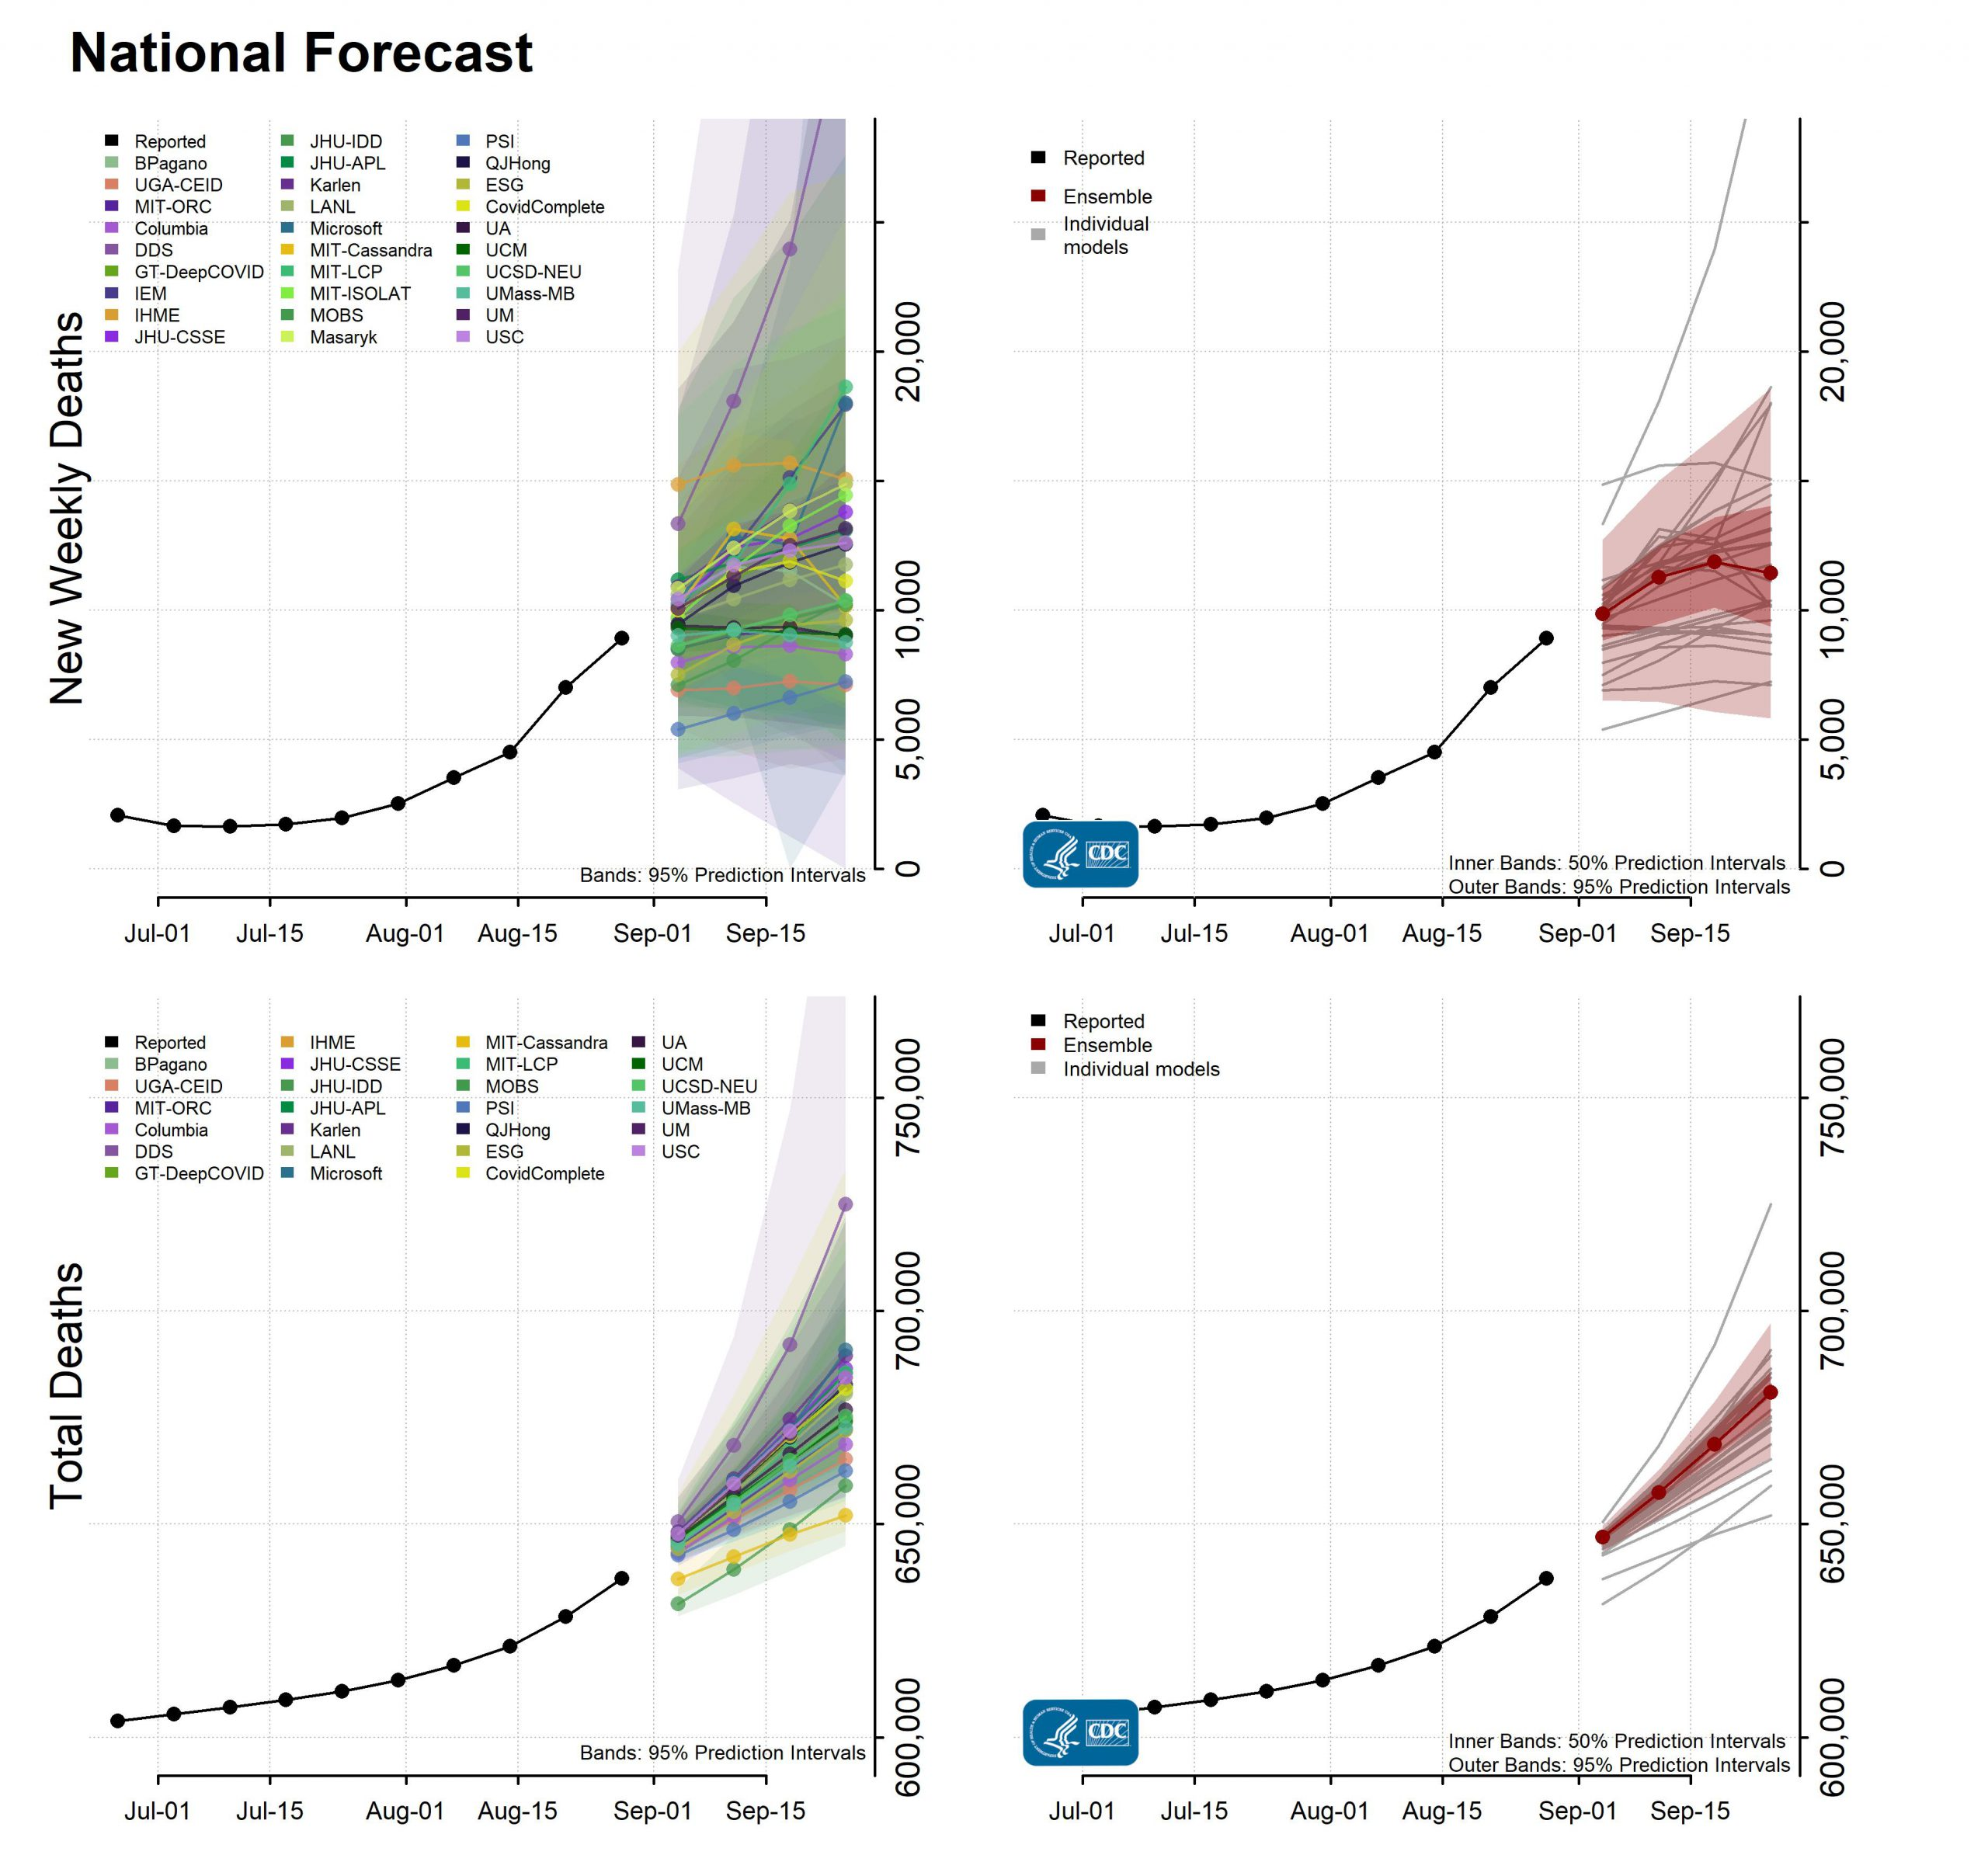
\includegraphics[scale=.24]{Images/8_30_21_cvd_deaths.jpeg}}
\begin{center}
\begin{minipage}{10cm}
\captionsetup{font=scriptsize}
\caption[Official CDC COVID-19 deaths report August 2021]{This image, 
published on www.cdc.gov in August 2021 as official public communication 
by the CDC, shows forecast models for national new weekly deaths due to COVID-19 
in the top row and cumulative deaths on the bottom row. The plots in the left 
column show prediction intervals from multiple teams whereas the plots on the 
right show the intervals for an ensemble forecast model with gray lines
predicting individual model point forecasts.}
\label{fig:cdcoff}
\end{minipage}
\end{center}
\end{figure}

\section{Outline}
In the context of collaborative forecasting like that of the CDC flu competition
or the COVID-19 Forecast Hub, bin forecasts and quantile forecasts have become
important representations to those involved in the projects. Yet both 
representation types come 
with their drawbacks. Computer
storage for instance might be a concern if many bin distributions are used for 
forecasting, 
and scoring methods are limited if forecasts are quantile forecasts.

In this paper, we propose the use of finite mixture distributions as a means 
of forecasting for collaborative projects similar to the CDC flu competition or 
the COVID-19
Forecast Hub. A finite mixture distribution -which we will refer to as a
\emph{mixture distribution}- is distribution constructed by combining a finite 
collection of other distributions. In this paper, we focus on the case where the
collection of distributions are parametric distributions.

In Section \ref{section:representations}, 
popular probabilistic forecast representation 
types are defined and reviewed. Methods of scoring, storing, constructing 
ensembles, and other aspects will be reviewed and compared for each 
representation type.
In Section \ref{section:conmixforc}, details for using mixture 
distributions in a collaborative forecast project are presented as well as tools
which may be used for scoring and constructing an ensemble.
Section \ref{section:retrostud} is a retrospective study of the CDC flu 
competition and COVID-19 Forecast Hub
forecasts and an attempt to assess whether forecast models
may be approximated by one component mixture distributions.






















\chapter{Probabilistic forecast representations}
\label{section:representations}

In this section we review four forecast representations already commonplace in 
forecasting. In a collaborative setting, certain aspects of each representation
should be considered including scoring, computer storage, and how to construct
an ensemble forecast. For each representation presented, applications of each of 
those aspects are also presented.


\section{Representation aspects to consider in collaborative projects}
\subsection{Scoring}
Scoring rules are used to numerically evaluate or \emph{score} a probability 
forecast. 
The
score is a measure of the accuracy of the forecast and where multiple forecasts
exist the score for each may be used to compare forecasts. If a scoring rule 
is \emph{proper}, then the best possible score is obtained by reporting the true 
distribution. The rule is strictly proper if that value is unique. 
Under proper
scoring rules, a forecaster has no incentive to be dishonest in their 
submission \cite[]{gneiting2007strictly}. This makes proper scoring rules ideal
for evaluating forecasts. We will limit our review of scoring methods to rules
which are proper.

\subsection{Storage}
For a collaborative forecast project where many researchers are involved and 
many predictions are collected, computer storage may need to be addressed. 
As an example of required computer storage, the 
repository for the
COVID-19 Forecast Hub contained 85 million forecasts as of 
April 4, 2022 which required more than 11.7 gigabytes of storage!
\cite[]{covidgithub}.
When determining the goals of a forecast project, there should be consideration 
of the storage required for different forecast representation types.

\subsection{Ensemble construction}
A multi-model ensemble is a statistical model made by combining information from
two or more individual statistical models. Private and public decisions are 
regularly made after combining information from multiple sources. For any given
situation, information from one source may provide insight on a subject which 
other
sources fail to capture. Likewise one statistical model may provide insight
that another model does not so that when they are combined into an ensemble the 
ensemble outperforms the individual component models.

As probabilistic forecasting becomes more commonplace, so too does ensemble 
modeling. Ensembles have been used extensively in weather and
climate modeling \cite[]{baran2018combining}, 
and they have been used increasingly in modeling infectious disease outbreaks
\cite[]{yamana2016superensemble}. 
Ensembles allow for an incorporation of multiple signals -
often from differing data sources- and sometimes individual model biases are 
canceled
out or reduced by biases from other models \cite[see references
therein]{reich2019accuracy}. 
In several disease outbreak studies, ensemble forecasts have been 
shown to outperform individual model forecasts
\cite[see
references therein]{ray2020ensemble, cramer2021evaluation}.

Construction of an ensemble may be done by combining individual forecast 
models using weighted averages. This has been called stacking 
\cite[]{wolpert1992stacked} or weighted density ensembles 
\cite[]{ray2018prediction}. 

\section{Probabilistic forecast representation types}
\subsection{Parametric distributions}
\label{section:pardist}
A parametric distribution is a discrete or continuous probability distribution 
described by a known function $p(x) := p(x|\theta)$. The function $p(x)$ is 
called a probability mass function (pmf) if the distribution is discrete and 
is called a probability density function
(pdf) if the distribution is continuous. Here $\theta$ is a vector of known or 
unkown parameters contained in the parameter space of the distribution. 

The value of $p(\cdot)$ evaluated at $x$ is defined as 
$p(x) = P(X = x)$ or the probability that the random variable $X$ takes
on $x$ in the space of the random variable. In the continuous case 
$P(X = x) = 0$ for all $x$, but the probability 
that $X$ falls within an interval $(a,b)$ is calculated by 
\eqref{equation:prob}.

\begin{equation}
\label{equation:prob}
  P(a < X < b) = \int_a^b p(x) dx
\end{equation}

Other functions classified by a parameteric distribution include the cumulative
distribution function (CDF) and the inverse CDF or quantile function. The CDF 
in the continuous case is defined in \eqref{eq:ccdf} and is defined in the 
discrete case in \eqref{eq:dcdf}. Here $x_n$ is the largest value of X less than 
or equal to $x$.
The quantile function is defined in \eqref{eq:quant} which returns a quantile 
value where $p$ is a given probability such that $0\leq p \leq 1$.

\begin{equation}
\label{eq:dcdf}
  F(x) = P(X \leq b) = \sum_{x \in X} p(x)
\end{equation}

\begin{equation}
\label{eq:ccdf}
  F(x) = P(X \leq b) = \int_{-\infty}^x p(t) dt
\end{equation}


\begin{equation}
\label{eq:quant}
  Q(p) = \inf \{ y \in \mathbb{R} : p \leq F(x) \}
\end{equation}



For a forecast represented as a parametric function with pmf/pdf $p_m(\cdot)$, 
the accuracy of the forecast may be measured by how likely realized value $x^*$
is to occur. Commonly used proper scoring rules for parametric distributions
include the logarithmic score (LogS), the
continuous rank probability score (CRPS) \cite[]{hersbach2000decomposition}
\cite[]{alves2013ncep}, and the interval/Brier 
score (IS) \cite[]{gneiting2007strictly} among 
others. See also \cite[]{gneiting2014probabilistic}
Section 3 for more on proper scoring functions. The definitions 
\eqref{eq:logs} and \eqref{eq:crps} are found in the review by Krueger.

For a forecast with pdf/pmf $p_m(\cdot)$, the LogS evaluates the 
probability of the observed value $x^*$. It is defined in \eqref{eq:logs}.

\begin{equation}
\label{eq:logs}
  LogS(p_m,x*) = -log\;p_m(x^*)
\end{equation}
The goal for a forecaster is to minimize the LogS, so a forecast $p^{'}_m(x^*)$ 
is considered 
superior to $p_m(x^*)$ if
$LogS(p^{'}_m, x^*) < LogS(p_m, x^*)$.
The LogS is limited to scoring forecasts with density functions and
evaluating those densities only at the point $x^*$.

The CRPS is a function of a CDF $F$
and so it may
be used more extensively than the LogS. 
For the CDF $F_m$, the CRPS is defined in \eqref{eq:crps}.
Here too a smaller score indicates a more accurate forecast.

\begin{equation}
\label{eq:crps}
  CRPS(F_m, x^*) = \int_{-\infty}^{\infty} (F_m(x)- 1_{\{x*\leq x\}})^2 dy
\end{equation}


Besides evaluating forecasts, the CRPS may also be used for optimizing weights 
used
to build ensembles under model averaging (MA). Considered the 
state-of-the-art techniques for combining 
component distributions
into an ensemble distribution are nonhomogeneous regression (NR), also known as
ensemble model output statistics (EMOS), and ensemble
MA, both of which are defined in \cite[]{gneiting2014probabilistic}.

In the context of an ensemble made from component models submitted from various
sources,
MA may be preferable because it does not require that modeling methods for 
individual components be the same. 
In MA, the final model does not have to be specified
beforehand and the resulting forecast will be a mixture distribution
of all component forecasts. The general form for an ensemble distribution $p^E$
is in \eqref{eq:bma}. Here $p_m$ is the $m^{th}$ component forecast 
distribution and 
$0 \leq w_m \leq 1$ is a weight assigned to that component where $\sum w_m = 1$.
Methods for estimating weights include maximum likelihood estimation
\cite[]{raftery2005using}, MCMC 
sampling \cite[]{vrugt2008ensemble},
and minimizing the CRPS of the ensemble
\cite[]{baran2018combining}.

\begin{equation}
\label{eq:bma}
  p^E(x) = \sum_{m=1}^M w_mp_m(x)
\end{equation}


For selecting distribution weights, minimizing the CRPS has some nice 
properties, but it can also be
difficult to compute. For example, when the forecast is a mixture of a 
truncated normal distribution (TN) and a truncated lognormal (TL) the CRPS is 
not available in closed form \cite[]{baran2018combining}.

Generally computation and evaluation of parametric distribution functions is not 
hard. 
For most commonly used parametric distributions -normal, lognormal, Poisson,
gamma, etc.- there is software readily available to compute density, 
distribution, and quantile values. 
A completely defined continuous parametric distribution may be evaluated at a
continuously
infinite number of values. We will call this an infinite resolution.
And requirements for storage are low 
compared to other representation types that will be discussed. The most common
parametric distributions can be fully defined with three or pieces of data
including
the distribution family and two parameters. Table \ref{table:pstor} 
contains
enough information to completely define a $\mbox{Lognormal(1,0.4)}$ 
distribution.

\begin{table}[h!]
\begin{center}
\begin{minipage}{10cm}
\captionsetup{font=scriptsize}
\centering
 \begin{tabular}{|c c c|} 
 \hline
 family & param1 & param2 \\ [0.5ex] 
 \hline
 lnorm & 1 & 0.4 \\ 
 \hline
 \end{tabular}
 \caption[Parametric distribution storage]{This is an example of data required
 for a lognormal 
 distribution with 
 parameters $\mu = $ 1 and $\sigma =$ 0.4}
 \label{table:pstor}
 \end{minipage}
 \end{center}
\end{table}


A drawback of representing a forecast in a parametric distribution is the lack 
of flexibility in the model selection. Easy computation and evaluation of these 
models is limited to what is available in software, so certain distributional
shapes may unattainable.
Requiring a parametric forecast also bars the use of some statistical methods
which might be used to create a forecast model including some Bayesian methods
where a posterior distribution cannot be computed in closed form.


\subsection{Sample distributions}
Forecast model builders may want more flexibility in modeling than a 
parametric 
distribution can provide. Methods that require sampling from a posterior 
distribution or Bootstrap sampling to obtain a sample distribution are examples
where parametric distributions may not be appropriate for modeling because of 
the lack of flexibility in distribution shape.

A sample distribution is made of a sample of random variables 
$(X_1,...,X_n)$ where $X_i \sim D$ and $D$ is some distribution. From this 
sample,
statistics such as mean, median, variance, and quantiles may be calculated. 
An empirical cumulative distribution function (ECDF) may also be calculated as
in \eqref{eq:ecdf}.

\begin{equation}
\label{eq:ecdf}
  ECDF = F_n(x) = \frac{1}{n} \sum_{i=1}^n \mathbb{I}(X_i \leq x)
\end{equation}

According to the Strong Law of Large numbers, the sample mean will converge to
the expected value of the distribution as $n \rightarrow \infty$ as long as the 
expected value of that distribution exists. Likewise by the same law the 
ECDF will converge to the true CDF 
as $n \rightarrow \infty$. Thus, if a sufficiently large 
sample is generated from a distribution with for which an expectation exists, 
the sample will closely approximate the 
true distribution. 

For common distribution families it is easy to generate large samples using 
existing functions in \texttt{R} and other programming platforms. For some 
distributions 
for which the mathematical formula is unkown or is not in closed form, more 
sophisticated methods may be required to generate samples. Bayesian analyses may 
require a Gibbs sampling or a Metropolis-Hastings algorithm, among others, 
to generate a 
sample. Such samples are useful in that the true distribution may be closely 
approximated without knowing the true mathematical form. 

Under the sample distribution representation, the options that a researcher has 
for constructing a forecast are more than
if they are asked to submit a parametric distribution, and the range of possible 
shapes for a distribution is larger.
In the last few decades, increased computing power and improvements in MCMC
sampling have greatly contributed to growth in the use of
sample distributions for forecasting \cite[]{gneiting2007strictly}
\cite[see examples listed therein]{krueger2016probabilistic}.

To properly score a forecast represented by a sample distribution, both the CRPS
and LogS may be used. The CRPS has the advantage here of scoring the sample 
distribution directly since the CDF in  (\ref{eq:crps}) may be replaced with the 
ECDF in
(\ref{eq:ecdf}). To use the LogS to score a forecast, a density function for the 
sample must be approximated. Common approximations include a kernel density (KD)
or Gaussian approximation (GA).

The KD in \eqref{eq:kd} is defined by Krueger et. al 
where $K$ is a kernel function, and $h_n$ is a suitable bandwidth. The GA is 
defined in \eqref{eq:ga} where $\Phi$ is the standard normal CDF and 
$\hat{\mu}_n$ and $\hat{\sigma}_n$
are the empirical mean and standard deviation of the sample $(X_i)$
\cite[see also for a comparison of scoring MCMC drawn forecasts between the CRPS 
and the LogS]{krueger2016probabilistic}.

\begin{equation}
\label{eq:kd}
  \hat{p}_n(x) = \frac{1}{n h_n} \sum_{i=1}^n K \left( \frac{x-X_i}{h_n} \right) 
\end{equation}

\begin{equation}
\label{eq:ga}
  \hat{F}_n(x) = \Phi  \left( \frac{x-\hat{\mu}_n}{\hat{\sigma}_n} \right)
\end{equation}




To build an ensemble model from sample distribution forecasts, the MA 
construction from (\ref{eq:bma}) may be used only replacing $p_m$ with the
approximate KD or GA pdf functions
-$\hat{p}_{n_m}^{KD}$ or $\hat{p}_{n_m}^{GA}$  
Here as well the optimal weights 
$w_m$ may be estimated by maximizing the likelihood or minimizing CRPS. 
If the desire is that the ensemble still be
a sample distribution, after selecting weights, a sample may be selected by 
randomly selecting a sample from $(X_n)_m$ with probability $w_m$.

A potentially large issue with using sample distributions is the amount of storage
it would require. For example when making MCMC draws from a posterior 
distribution, the final sample distribution can have a sample size of thousands
or tens of thousands. Maybe not all distributions would require such a large 
sample size, but sizes of at least dozens or hundreds would be required for each
forecast prediction. For any project the size of the CDC flu competition or the
COVID-19 Forecast Hub, the storage required would be large and potentially 
expensive.

\subsection{Bin distributions}
An alternative to parametric distributions and sample distributions which allows
for higher flexibility in distribution shape than a parametric distribution and 
will usually require less storage space than samples is a bin 
distribution.

A bin distribution may be constructed over a set 
$A = [a, b)$ by partitioning $A$ into a set of $K$ bins $\{B_i\}_{i=1}^{K}$
where $B_i = [b_{i-1}, b_i)$ and $\cup_{i=1}^{K} B_i = A$. Based on the problem
to be forecasted, researchers will determine the possible range $A$ and 
select the number of bins and the sizes for each bin. It may be the case
that a collaborative project will set the width of all bins to be equal so that 
$\Delta = b_i - b_{i-1}$ is the same width for all $i$ 
\cite[]{mcgowan2019collaborative}.
To complete the construction, a probability $p_i$ is assigned to each $B_i$ 
where $\sum_{i=1}^{K}p_i = 1$. These probabilities are determined by the 
forecasters. 
This representation with a given bin and assigned probability may be 
treated like a discrete distribution with a pmf in that the calculations of 
moments and of the 
the cumulative distribution are done the same as for a discrete parametric 
distribution. For a random variable $X$ from a binned distribution 
the $j^{th}$ moment may be calculated as in \eqref{eq:bev}. 
Here $\beta_i$ is a value corresponding to bin $B_i$ (such as $\beta_i = b_i$,
$\beta_i = b_{i-1}$ or $\beta_i$ is the mean or mid value in $B_i$). The 
cumulative distribution may be calculated as in \eqref{eq:bcdf}.
Here $p_n$ is the probability for the bin $B_n$ where $b \in B_n$.

\begin{equation}
\label{eq:bev}
  EX^j = \sum_{i=1}^n \beta_i^j p_i
\end{equation}


\begin{equation}
\label{eq:bcdf}
  P(X \leq b) = \sum_{i=1}^n p_i
\end{equation}


If the value to be forecasted takes on discrete values a common discrete 
distribution, such as a binary or Poisson distribution, may sometimes be used to 
assign probabilities to each of the bins. When the values to be forecasted are
continuous, a forecaster may need to employ a method of discretization to a 
forecast distribution. There are a number of possible ways to do this including
those outlined by Chakraborty and Subrata \cite[]{chakraborty2015generating}.

The CDC flu competition has used a bin distributions as the forecast 
representation. The CDC has also used it for other disease outbreak
forecast projects.
In that context it has become the standard representation 
\cite[]{brooks2020comparing}. Much work has been done in evaluating 
and constructing ensemble models on influenza forecasts represented by 
discretized bins 
\cite[]{mcgowan2019collaborative, mcandrew2019adaptively,reich2019collaborative}. 

Because discretized bins can be seen as a pmf, methods for proper scoring 
already 
discussed -LogS and CRPS- are useable and MA is valid method for ensemble 
construction. Reich et. al used MA to combine multiple forecasts from the flu 
competition. They built and compared ensemble models with different weighting
schemes including equally weighted components $w_j = 1/J$ and estimating weights
according to the model specification. To estimate weights they used the 
expectation maximization (EM) algorithm 
\cite[see
supplementary material within for details]{reich2019accuracy}.

The exact amount of information required for a discretized bin forecast will 
vary depending on the permitted range of the forecast and the desired 
resolution. 
In the CDC flu contest, a forecast might have 131 bins between 0\% and 13.1\% 
-bins having increments of 0.1 or 0.01\%- with 
corresponding probabilities in each. This makes 262 pieces of information per
prediction. For any binning scheme of more than two bins, the information 
requirement for bin distributions will be higher than for parametric 
distributions.
Table \ref{table:dbins} illustrates what a discretized 
$\mbox{Lognormal(1,0.4)}$ distribution truncated over $[0,8]$
looks like in 41 equally spaced bins. The discretization was done
such that the probabilities $p_i$ are calculated as in \eqref{eq:disc}
where $p^{TL}$ is the pdf of a truncated $\mbox{Lognormal(1,0.4)}$. This is 
similar
to Methodology-IV from Chakraborty 
\cite[]{chakraborty2015generating,kemp2004classes}.

\begin{equation}
\label{eq:disc}
  p_i = \int_{b_{i-1}}^{b_i} p^{TL}(x) dx
\end{equation}


Submitted as a forecast prediction, the distribution illustrated in table 
\ref{table:dbins} 
includes 82 pieces of data. For parts 
of the CDC influenza competition some forecasts included up to 262. This is 
far less storage than the possible thousands of draws from a sample 
distribution but is 
still much larger than the three or five data pieces required to report a 
lognormal
or truncated lognormal distribution.

\begin{table}[h!]
\begin{center}
\begin{minipage}{10cm}
\captionsetup{font=scriptsize}
\centering
 \begin{tabular}{|c|c|} 
 \hline
    bin & prob \\ \hline
    ... & ... \\
    {[1.4,\;1.6)} & 0.04414 \\
    {[1.6,\;1.8)} & 0.05896 \\
    {[1.8,\;2.0)} & 0.07032 \\
    {[2.0,\;2.2)} & 0.07172 \\
    {[2.2,\;2.4)} & 0.07955 \\
    ... & ... \\
 \hline

 \end{tabular}
  \caption[Discretized bin distribution storage]{This is a storage example of a
  discretized
  lognormal with $\mu = 1$ and $\sigma = 0.4$ truncated over $[0,8]$.}
\label{table:dbins}
\end{minipage}
\end{center}
\end{table}



Besides potentially large amount of information required per forecast,
creating the right 
binning scheme may be a challenge. Because there must be a finite number of
bins, forecast distributions often have a finite support. And where the range of 
possible outcomes to a problem is not well known, the right binning scheme may 
be
hard to produce. This may depend on the details of the event to be forecasted, 
but in the case of the COVID-19 outbreak choosing the right set of bins posed
a few problems.









\subsection{Quantile representation}
When deciding how forecasts should be represented in the COVID-19 Forecast Hub,
the time pressure of generating forecasts and the large
range for possible outcomes both contributed to the COVID-19 Forecast Hub 
decision
to forego trying to create the right binning scheme and use quantile forecasts
to forecast the COVID-19 pandemic \cite[]{bracher2021evaluating}.
The COVID-19 Forecast Hub requires predictions to be submitted as 11 or three 
nominal 
intervals -depending on the specific target and unit to forecast- and a median.
Using this interval or quantile representation leads to a number of changes in 
the scoring and ensemble building of forecasts.

A quantile forecast is constructed as in \eqref{eq:quantiles}.
Here for $N$ given quantiles $\alpha_1,..., \alpha_N$; $q_1,..., q_N$ are the 
values such that 
When the quantiles are reported as prediction intervals we have 
\eqref{eq:intervals}.

\begin{equation}
\label{eq:quantiles}
  P(Y \leq q_1) = \alpha_1, P(Y \leq q_2) = \alpha_2, ..., 
  P(Y \leq q_N) = \alpha_N
\end{equation}


\begin{equation}
\label{eq:intervals}
  P(Y \leq q_1) = \alpha_1, P(Y \leq q_2) = \alpha_2, ...,
  P(Y \leq q_{N-1}) = 1 - \alpha_2, P(Y \leq q_N) = 1 - \alpha_1
\end{equation}

What is possible for scoring forecasts
or constructing ensemble in other representations is often not possible with
quantile forecasts. The shape of a distribution is also not known and in fact,
nothing is known about the tails or the uncertainty beyond the most 
extreme reported quantile values. In the COVID-19 Forecast Hub predictions, 
nothing 
is reported about the range below the $1^{st}$ quantile or above the $99^{th}$.
Yet the quantile representation has its advantages. 

Quantile forecasts allow for forecasters to submit fairly detailed
forecasts without restricting the range of possible values.
Since quantiles are easily calculated from any regular distribution type
-using the quantile function for parametric functions or calculating sample 
quantiles- we consider quantile forecasts to be highly flexible in terms of 
what methods forecasters may employ in modeling.

To score a quantile forecast, 
neither the LogS nor the CRPS may be used, 
but another proper scoring rule the IS may be used.
For an observed outcome $x^*$ and a prediction interval $(l,r)$ 
where $l$ and $r$ are the $\alpha/2$ and $(1-\alpha/2)$ quantiles that bound
the central $(1-\alpha)$ prediction interval the IS is defined in \eqref{eq:is}.
This is a sum -weighted by 
$\alpha$- of the width of the
interval and the distance between $x^*$ and the interval (if $x^*$ is not 
captured in the interval) \cite[]{gneiting2014probabilistic}. 
The IS requires only a single central 
$(1-\alpha) \times 100$ prediction interval.

\begin{equation}
\label{eq:is}
  IS_{\alpha}(l,r; x^*) = (r-l) + \frac{2}{\alpha}(l-x^*)1\{x^*<l\} 
  + \frac{2}{\alpha}(y-r)1\{x^* > r\}
\end{equation}


When an quantile forecast is made up of multiple intervals each with different
$\alpha$ levels, the weighted interval score (WIS) may be used as it was by
Bracher et.
al use the WIS to score COVID-19 quantile forecasts 
\cite[]{bracher2021evaluating}.
There are multiple versions of the WIS -some of 
which are described in Bracher et. al, but the version used by the COVID-19 
Forecast
Hub for a forecast of $K$ intervals is defined in \eqref{eq:wis}.
Here $median$ refers to the predictive median and $w_k = \alpha_k/2$ is the 
weight on the $k^{th}$
interval. With that selection of weights, it may be shown that the
WIS approximates the CRPS \cite[see S1 Text therein]{bracher2021evaluating}.

\begin{equation}
\label{eq:wis}
  WIS_{0,K}(F_m,x^*) = \frac{1}{K + 1/2} \times (w_0, \times |x^*-median|+
  \sum_{k=1}^K \{ w_k \times IS_{\alpha_k}(F_m,x^*) \} )
\end{equation}


Bogner, Liechti and Zappa compared scoring forecasts of quantiles with the 
Quantile Score (QS) similar to the interval score and scoring distribution functions
fit to those quantiles using the CRPS \cite[]{bogner2017combining}. The CRPS 
corresponds to the integral of the QS over all possible thresholds rather than
just specific quantiles, so it more effectively reveals deficiencies in parts of 
the distribution and especially in the tails past the end points of quantiles
used in QS or IS. Thus there may be something lost in terms of scoring when the 
WIS is used.

Like the CRPS, not only does the WIS provide an easily interpretable proper 
score for interval forecasts, but it may also be useful when building an 
ensemble forecast.
The ensemble forecast constructed by the COVID-19 Forecast Hub was made as an
equally-weighted average of forecasts from the component models. More 
specifically, each quantile value of the ensemble was the average of values from
all models corresponding to the same quantile \cite[]{ray2020ensemble}. For $M$ 
models each with $K$ quantiles, the $k^{th}$ ensemble quantile $q^E_k$ is 
calculated as in \eqref{eq:qa}
where $\nu_m$ is the weight assigned to each forecast and $\sum \nu_m = 1$. In
the COVID-19 Forecast Hub model, $\nu_m = \nu = 1/M$. Where the overall mean or 
a weighted mean may be used, the median may also be used.
Brooks et. al compare performance of the COVID-19 ensemble
using equally-weighted means, weighted means, and median value constructions
\cite[]{brooks2020comparing}.
In their report, they show that weighted means and median constructions tend
to outperform an equally-weighted mean construction. To come up with optimal 
weights, they select values $\nu_m$ from (\ref{eq:qa}) which minimize the WIS of 
the ensemble forecast.


\begin{equation}
\label{eq:qa}
  q^E_k = \sum_{m=1}^M \nu_m q_k^m 
\end{equation}



Quantile averaging or Vincentization for a complete distribution is defined as
in \eqref{eq:vinc}
where $F_m^{-1} (\alpha) = \inf \{y:F_m(y) \geq \alpha\}$ for 
$0 < \alpha \leq 1$. Some notable characteristics are that it is more likely for
the ensemble distribution
to be unimodal than it is under linear averaging of densities like MA 
\cite[]{busetti2017quantile}. Under some circumstances, such as when member
distributions are exponential, Weibull, or logisitic the aggregated distribution
is of the same family \cite[]{ratcliff1979group}. Quantile averagin produces 
smoother
distributions than MA according to Schepen and Wang \cite[]{schepen2015model}.
And Lichtendahl et. al conclude that quantile averaging produces sharper 
forecasts
and tends to perform better in scoring than probability averaging, MA,
\cite[]{lichtendahl2013better}.

\begin{equation}
\label{eq:vinc}
  F_v^{-1}(\alpha) = \sum_{m=i}^M w_m F_m^{-1} (\alpha)
\end{equation}


As in sample distributions and bin distributions, 
data storage for interval forecasts will
depend on the desired clarity of resolution. For the COVID-19 forecasts 
submitted to the COVID-19 Forecast Hub, 23 quantile values are requested for 
quantiles (0.01, 0.025, 0.05, 0.10, …, 0.95, 0.975, 0.99). This includes a 
median along with 11 predictive intervals \cite[]{bracher2021evaluating}. 
Forecasters are thus required to submit 46 values in each short-term forecast 
(some of the longer term forecasts only include seven quantiles). In terms of 
storage, this is an improvement over requirements for the flu contest. Table
\ref{table:qstor} shows what a submission of 23 quantiles from a 
$\mbox{Lognormal(1,0.4)}$ might look like.



\begin{table}[h!]
\centering
\begin{center}

\captionsetup{font=scriptsize}

 \begin{tabular}{|c||c|c|c|c|c|c|c|c|c|}
 \hline
    quantile & 0.01 & 0.025 & 0.05  & ...  & 0.95 & 0.975 & 0.99 \\ \hline
    value & 1.07137 & 1.2404 & 1.40689 & ... & 5.18328 &
    5.82391 & 6.58783 \\
    
 \hline
 \end{tabular}
 \begin{minipage}{10cm}
 \caption[Quantiles and values storage]{This shows six quantiles
 and values from a lognormal distribution with $\mu = 1$ and $\sigma = 0.4$}
 \label{table:qstor}
 \end{minipage}
 \end{center}
\end{table}

Figure \ref{fig:denscomp} illustrates how the densities and CDFs compare 
between parametric distributions, sample distributions, bin distributions, and
quantiles. 

\begin{figure}[htbp]
\begin{center}

\captionsetup{font=scriptsize}
\centerline{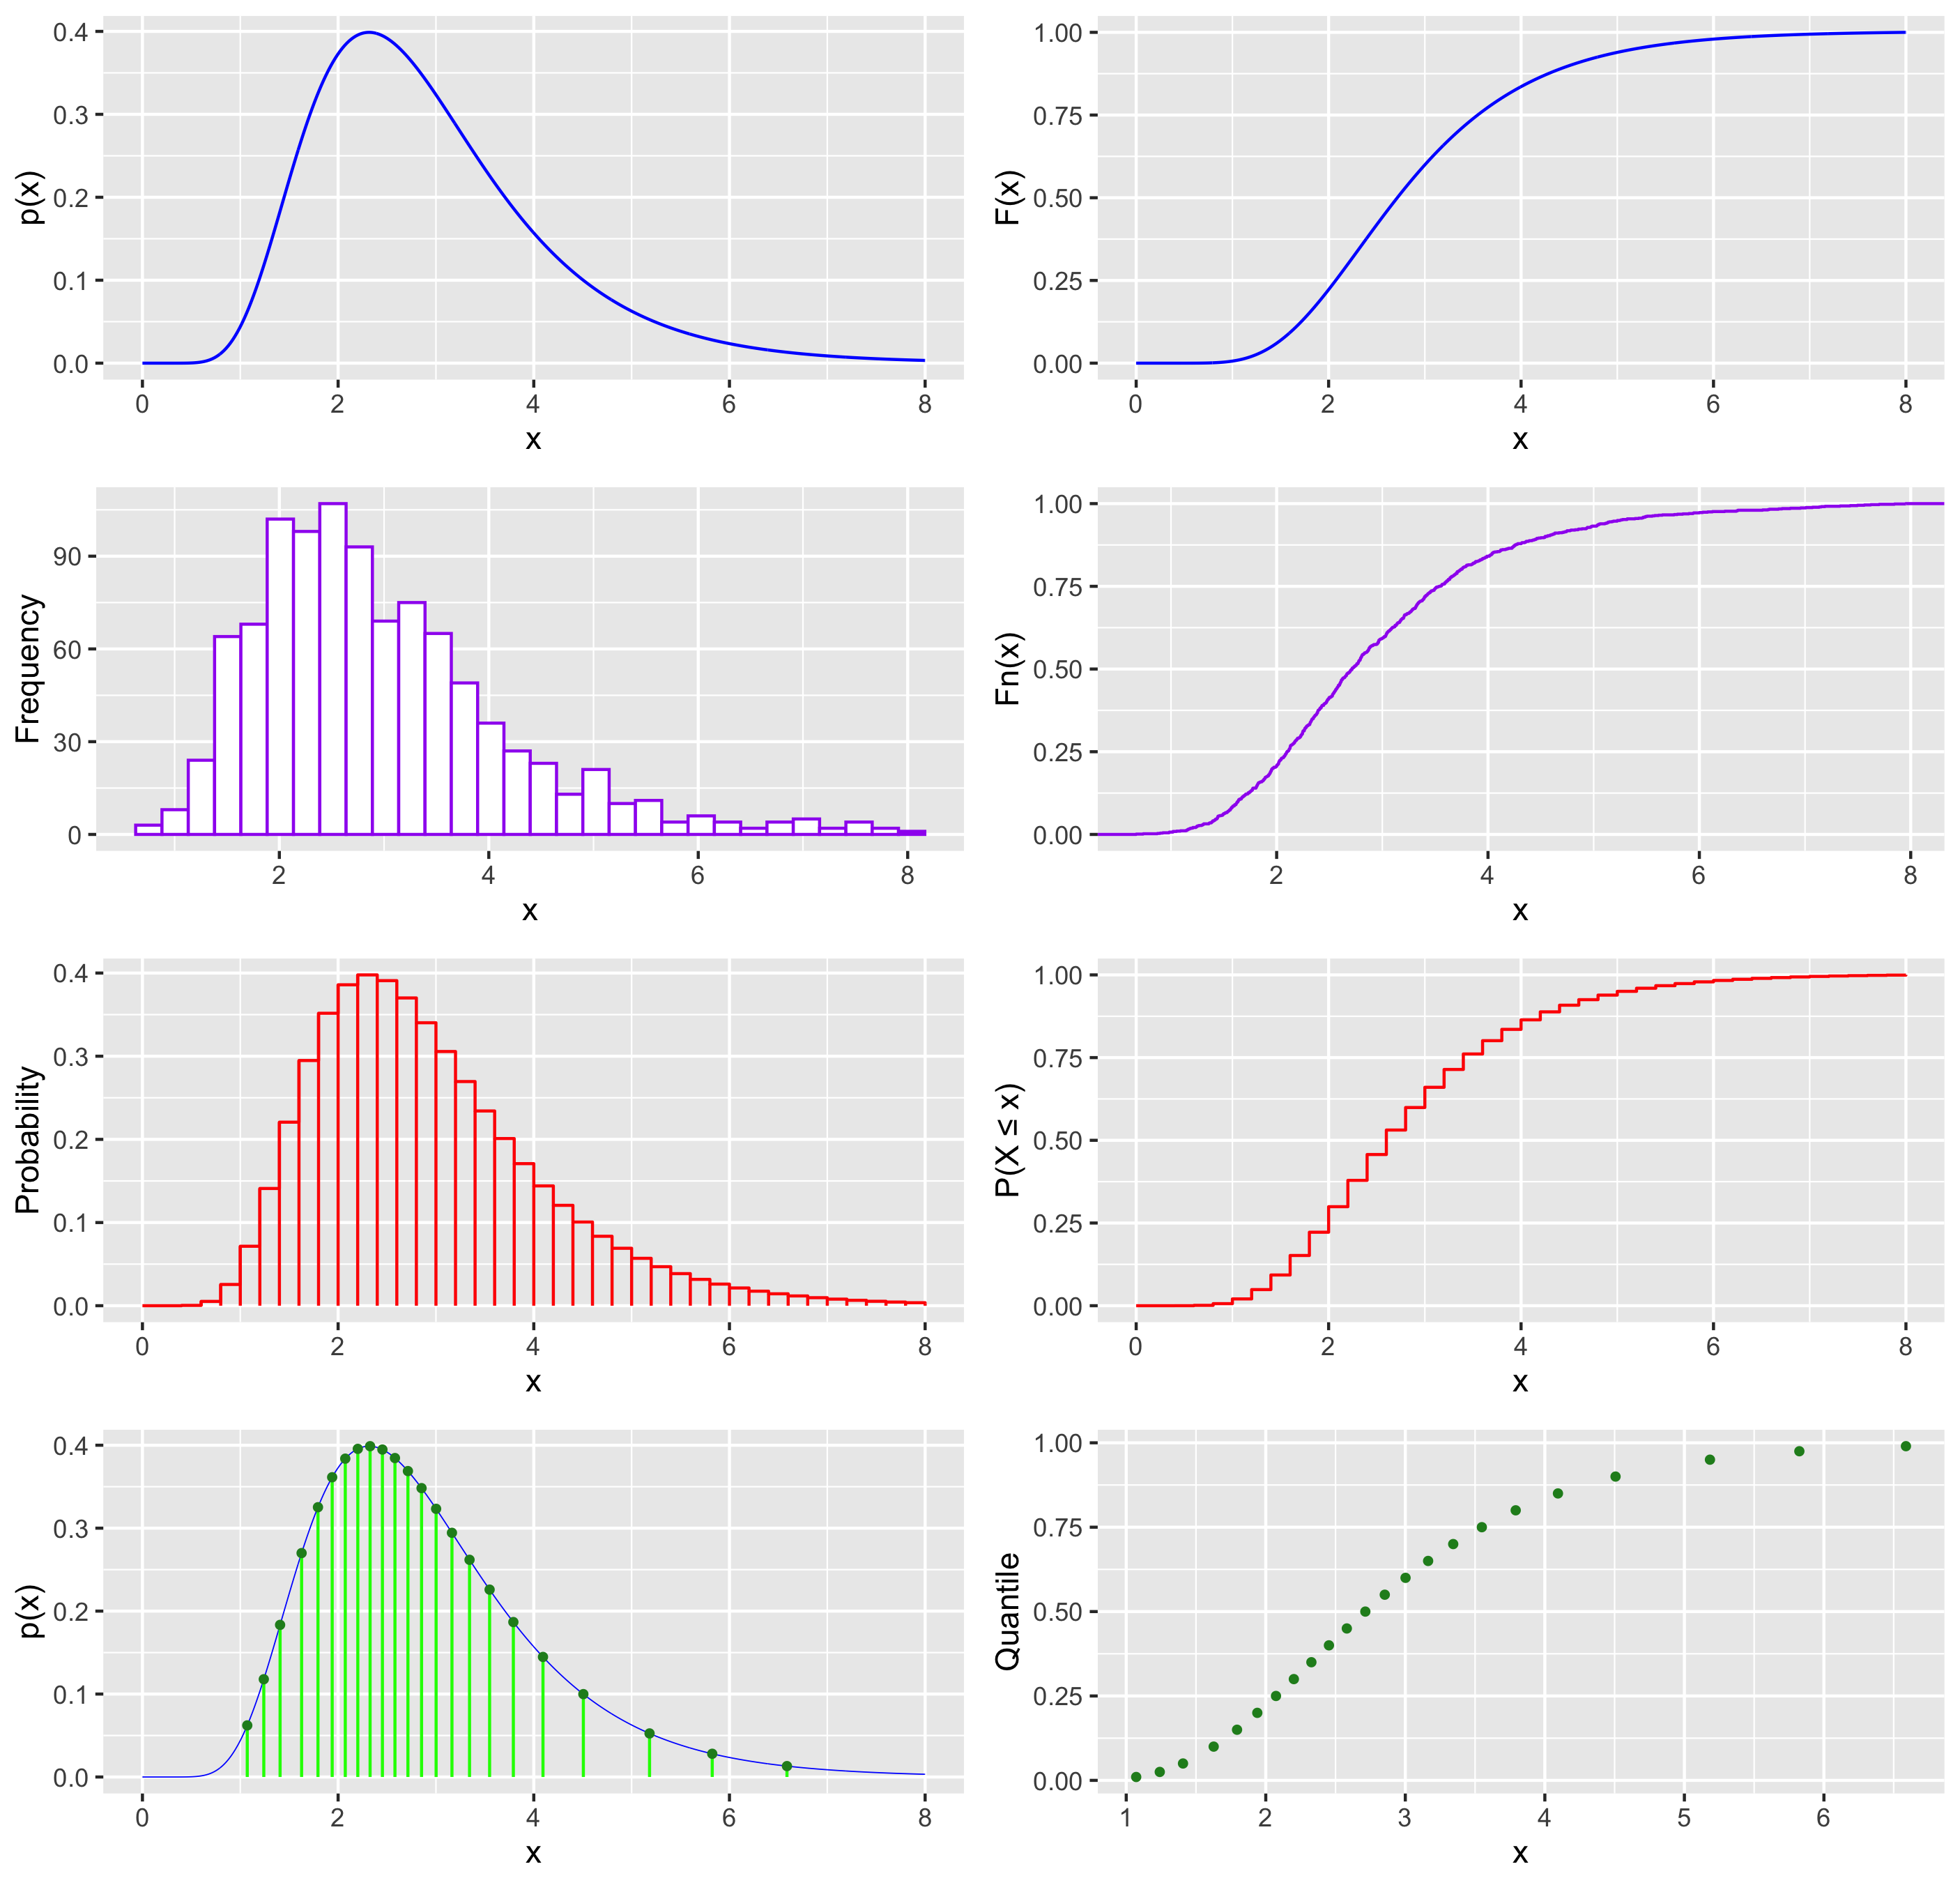
\includegraphics[scale=.1]{Images/dens_cum_comp.png}}
\begin{minipage}{10cm}
\caption[Density/CDF comparison between parametric distribution, sample 
distribution, discretized bin distribution and quantiles]{This figure compares 
the
densities and CDFs of forecast representation types discussed in the left and 
right columns respectively. Each is generated from a Lognorma(1,0.4) 
distribution. Blue shows the density and CDF functions. Purple shows a 
histogram and ECDF of 1,000 samples. Red shows bin probabilities and the CDF
function for a bin distribution. Green shows quantiles
with corresponding values.}
\label{fig:denscomp}
\end{minipage}
\end{center}
\end{figure}


\newpage

\section{Mixture distributions}
A mixture distribution forecast representation is an
attractive alternative to the four representations already discussed. 
A mixture distribution forecast
would allow for many distribution shapes, a high resolution, storage comparable
to that of bin and quantile forecasts, and the more common methods for scoring
and ensemble construction may be used.

A mixture distribution may be constructed in the same way as the
ensemble described in section \ref{section:pardist} 
(\ref{eq:bma}) 
where for $T$ distributions
with pdfs $p_t(x)$ and $z_t > 0$ and $\sum_{t=1}^{T} z_t = 1$ we have 
\eqref{eq:dmd}.
 

\begin{equation}
\label{eq:dmd}
  p^{M} = \sum_{t=1}^T z_tp_t(x)
\end{equation}




Like the parametric, a mixture distribution may be evaluated with
existing software like \texttt{distr} package in \texttt{R} 
\cite[]{camphausen2007distr}. 
And 
scoring may be done  
using the LogS, CRPS and IS. A mixture distribution, like its parametric 
distribution components, has an infinite resolution.

A mixture distribution may be much more flexible than a single component 
parametric distribution in 
terms of distributional shape. According to 
McLachlan and Peel, a mixture of 
normal densities with common variance can be used to approximate arbitrarily 
well
any continuous distribution \cite[]{peel2000finite} (see also 
\cite[]{nguyen2019approximations}). Thus, for an unconventional probability
distribution -such as MCMC posterior samples- it may be reasonable to 
approximate the distribution by fitting those samples to a mixture of normal
distributions.
Depending on the number of components a forecaster includes in a mixture 
forecast, the amount of storage per forecast might be as little as for a 
parametric forecast or as permitted in the specific forecast project. 

An ensemble model may be built by using \eqref{eq:bma} only replacing $p_m$
with $p_m^M$ in \eqref{eq:dmd}. Solving for weights may also be done by 
maximizing
the likelihood of the forecast or minimizing the CRPS. However with the 
added complexity of component models being mixture distributions the 
computation is likely to be more expensive. An example where this is
true is when trying to minimize the CRPS but the exact mixture doesn't 
produce a closed form CRPS \cite[]{baran2018combining}. In large projects like
the COVID-19 Forecast Hub, if an equal weight is not assigned to each component,
it may be determined that models not reaching a certain standard of predictive
performance are
assigned an ensemble weight of 0. This would simplify an ensemble model to 
include only the best performing forecasts.



Table \ref{table:repscomp} shows how a mixture distribution forecast 
compared with the other formats discussed in terms of methods for scoring,
information and resolution provided, methods for ensemble building, and computer
storage requirement. To summarize, a continuous mixture distribution has the 
infinite resolution of a parametric distribution with the flexibility of a bin
distribution, a sample distribution, and a set of quantiles. The common proper
scoring rules LogS and CRPS may be used to score it. The storage requirement is
comparable to that of a bin distribution or a set of quantiles. And MA may be 
used for building an ensemble.
In Section
\ref{section:conmixforc} we show how a mixture distribution may be constructed,
scored and used to construct an ensemble using software available in 
\texttt{R}.





\begin{flushleft}

  \begin{table}
   \begin{adjustwidth}{-1cm}{-1cm}
    \begin{tabular}{ | p{2.9cm} || p{3cm} | p{4cm} | p{3cm} | p{3.5cm} |}
    \hline
    \textbf{Representation} & \textbf{Scoring} & 
    \textbf{Flexibility/Information} & \textbf{Ensemble} &
    \textbf{Storage Requirement}
    \\ \hline \hline

    Parametric distribution & LogS, CRPS, IS & Limited to common 
    distribution families. 
    Infinite resolution
    & MA & Low 3-6 values per prediction \\ \hline
    
    Sample distribution & CRPS and IS. LogS after smoothing & Any shape. 
    Resolution may be
    very high but depends on sample size & MA after smoothing. Resampling 
    otherwise & 
    Hundreds or thousands of values per prediction
    \\ \hline
    
    Bin distribution & LogS, CRPS, IS &
    Any shape allowed, but limited by binning scheme. Range also may be limited
    & MA &
    Depends on binning scheme but dozens to hundreds of values
    \\ \hline


    Quantiles & IS, WIS & Shape unknown but with enough quantiles there is still
    a decent amount of information. No tail information & 
    Quantile averaging & Depends on 
    requested quantiles. Perhaps dozens of values
    \\ \hline
    
    Mixture distribution & LogS, CRPS, IS. May be more limited by computation & 
    With
    enough component distributions may
    approximate any distribution shape. Infinite resolution& MA 
    & 3 values to dozens per forecast depending on number of components
    \\ \hline
    
  
   
	 \end{tabular}
	 \end{adjustwidth}
	  \begin{center}
    \begin{minipage}{14cm}
    \captionsetup{font=scriptsize}
   \caption[Forecast representation comparison]{This table compares scoring,
   information, ensemble building, and storage requirements for the different
   forecast representations discussed. To summarize 
   a continuous mixture distribution has the 
infinite resolution of a parametric distribution with the flexibility of a bin
distribution, a sample distribution, and a set of quantiles. The common proper
scoring rules LogS and CRPS may be used to score it. The storage requirement is
comparable to that of a bin distribution or a set of quantiles. And MA may be 
used for building an ensemble.}
   \label{table:repscomp}
   \end{minipage}
   \end{center}
   \end{table}
	 
\end{flushleft}



























\chapter{Mixture distributions in a collaborative forecast project}
\label{section:conmixforc}


The CDC flu competition and the COVID-19 Forecast Hub as well as other 
collaborative projects
have their own established systems for receiving, 
scoring, and constructing ensemble forecasts. A transition from using bin or 
quantile forecasts to using mixture distribution forecasts
would require
a few adjustments to those systems. In this section we outline how some of these
adjustments may be implemented as well as present some tools which may be used
to build forecasts from submissions, score those forecasts, and construct 
ensembles from them.

\section{Submission format}
For a collaborative forecast project to run smoothly, forecast submissions from 
all forecasters 
should follow the same format. For both the CDC flu competition and
the COVID-19 Forecast Hub, teams provide a \texttt{.csv} spreadsheet which 
contains the distributional information for one or multiple forecasts. Tables
\ref{table:dstan} and \ref{table:qstan} show what variables are included and a
couple rows to illustrate possible values.
The column variables include \texttt{location}, \texttt{target}, \texttt{type},
\texttt{unit}, \texttt{bin} or \texttt{quantile}, and \texttt{value}.
Here \texttt{location} defines the specific county, state, or country of the 
forecast. The \texttt{target} variable defines what is forecasted with levels
season onset, deaths, hospitalizations, etc. The \texttt{type} variable defines
the type for the \texttt{value} variable with levels of \texttt{point}, 
bin, or quantile.
The \texttt{unit} variable defines the time frame of the forecast with levels of
week,
two weeks, four weeks, etc. The variables \texttt{bin} and \texttt{quantile}
give a specific bin or a specific quantile. And the \texttt{value} variable is a 
number that 
either gives the probability associated with a bin or the value associated 
with a quantile.

A single submission may include many forecasts aimed at forecasting a 
different combinations of \texttt{location}, \texttt{target}, and \texttt{unit}. 
A set of rows which share
the same specific combination of \texttt{location}, \texttt{target}, and 
\texttt{unit} constitute a single forecast. One forecast for the CDC flu
competition may require up to 131 rows whereas in the COVID-19 Forecast Hub one 
forecast may require up to 23 rows.


\begin{table}[h!]
\begin{center}
\begin{minipage}{10cm}
\captionsetup{font=scriptsize}
\centering
 \begin{tabular}{|c|c|c|c|c|c|}
 \hline
    location & target & type & unit & bin & value  \\ \hline
    % US National & Season Onset & Point & week & NA & . \\
    us national & season onset & bin & week & 0.0 & . \\
    us national & season onset & bin & week & 0.1 & . \\
    ... & ... & ... & ... & ... & ... \\
 \hline
 \end{tabular}
 \caption[Influenza competition submission example]{This shows a few rows of a 
 submission file
 for a discretized forecast like those in the CDC influenza forecast 
 competition. A set of rows which share the same combination of 
 \texttt{location}, \texttt{target}, and \texttt{unit} make up a
 single forecast. One submission may include many forecasts specified by 
 differing combinations of those three columns.}
 \label{table:dstan}
 \end{minipage}
 \end{center}
\end{table}



\begin{table}[h!]
\begin{center}
\begin{minipage}{11cm}
\captionsetup{font=scriptsize}
\centering
 \begin{tabular}{|c|c|c|c|c|c|}
 \hline
    location & target & type & unit & quantile & value  \\ \hline
    % US National & Season Onset & Point & week & NA & . \\
    us national & season onset & quantile & week & 0.01 & . \\
    us national & season onset & quantile & week & 0.025 & . \\
    ... & ... & ... & ... & ... & ... \\
 \hline
 \end{tabular}
 \caption[COVID-19 Forecast Hub competition submission example]{This shows
 a few rows of a 
 submission file
 for a quantile forecast like those in the COVID-19 Forecast Hub. 
 A set of rows which share the same combination of 
 \texttt{location}, \texttt{target}, and \texttt{unit} make up a
 single forecast. One submission may include many forecasts specified by 
 differing combinations of those three columns.}
 \label{table:qstan}
 \end{minipage}
 \end{center}
\end{table}



Table \ref{table:mstan} illustrates adjustments made to the submission formats
from 
Tables \ref{table:dstan} and \ref{table:qstan} which make a useable submission 
format for mixture distribution forecasts. In such a format, each row represents
a component used in a mixture distribution.
The variables \texttt{bin} or \texttt{quantile} and \texttt{value} are removed 
and replaced with \texttt{family},
\texttt{param1}, \texttt{param2}, and \texttt{weight} where \texttt{family} is 
the distribution family of the component,
\texttt{param1} and \texttt{param2} are the parameters for the component 
distribution, and \texttt{weight} is the 
weight $w_i$ for that component.

\begin{table}[h!]
\centering
 \begin{tabular}{|c|c|c|c|c|c|c|c|c|}
 \hline
    location & target & type & unit & family & param1 & param2 & weight
    \\ \hline
    us national & season onset & dist & week & norm & $a_n$ & $b_n$ & $w_1$\\
    us national & season onset & dist & week & lnorm & $a_l$ & $b_l$ & $w_2$\\
    ... & ... & ... & ... & ... & ... & ... & ...\\
 \hline
 \end{tabular}
 \begin{minipage}{11cm}
\captionsetup{font=scriptsize}
 \caption[Mixture distribution forecast submission example]{This is an example 
 of a 
 submission file
 for a disease outbreak forecast using a mixture distribution representation.
 Each row represents a component of a mixture distribution. The variables
 location, target, and unit specify what is being forecasted. The variable type
 specifies that the row represents a parametric distribution. The variables
 family, param1, and param2 specify the exact distribution. And the variable 
 weight specifies the weight $w_i$ that the component distribution has in the
 mixture distribution. Here two components are shown with distributions
 Normal$(a_n, b_n)$, Lognormal$(a_l, b_l)$ and weights $w_1$ and $w_2$.}
 \label{table:mstan}
 \end{minipage}
\end{table}

For reasons of storage and computation, a forecast project may have a limit to 
the number of components allowed per forecast.
For reference, a mixture distribution forecast following the 
format in table \ref{table:dstan} with 17
components would require $17 \times 8 = 136$ cells submitted per forecast. 
A submission to the COVID-19 Forecast Hub forecast 23 quantiles
according to the format in table \ref{table:dstan} requires
$23 \times 6 = 138$ cells. Thus if the COVID-19 Forecast Hub were to change the
forecast representation from quantile forecasts to mixture forecasts but 
continue allowing the same amount of data per forecast, 
a mixture distribution with 17 components could be used in one forecast. That
many components could allow for a large range of distribution shapes and 
flexible forecasts.

Throughout the remainder of this section, explanations of how to work with 
mixture distributions submitted according to Table \ref{table:mstan} is 
given. Also given is
\texttt{R} code which 
demonstrates constructing a mixture distribution from a forecast submission, 
scoring the forecast, and building an ensemble from two separate submissions.

\section{Mixture construction and scoring tools}
\label{section:tools}

A single \texttt{.csv} submission file of the format in Table \ref{table:mstan} 
may contain multiple forecasts forecasting different combinations of location,
target, and unit. Selecting only rows which share a specific combination of 
location, target, and unit will produce a table representing a single forecast.
That table may look like Tables \ref{tab:preddf1} and 
\ref{tab:preddf1}. If the table is saved as a standard \texttt{data.frame} in 
\texttt{R}, then tools based on the \texttt{distr} package 
\cite[]{camphausen2007distr} may be used for evaluating a mixture distribution 
with the components in the table. 


The \texttt{distr} package contains a function 
\texttt{UnivarMixingDistribution()} takes as arguments a list of distributions
and a vector of weights for each distribution and a object of class 
\texttt{AbscontDistribution} is returned. An \texttt{AbscontDistribution} class
is a mother class which defines a random number generator, pdf,
CDF, and quantile function for continuous distributions from common
families contained in the \texttt{distr} and for mixture distributions with 
component distributions from those families.
We wrote a function \texttt{MakeDist()} (see APPENDIX)
which takes on a \texttt{data.frame} with variables
family, param1, param2, param3, and weight and where each row represents a
component distribution in a mixture distribution. The function 
\texttt{MakeDist()} calls on the \texttt{UnivarMixingDistribution()} function
and returns a mixture distribution object of class \texttt{AbscontDistribution}.

If a forecast such as in Table \ref{tab:preddf1} is taken as an argument in 
\texttt{MakeDist()}, the resulting mixture distribution may then be evaluated 
with functions for the pdf, CDF, quantile function, and random samples from the
mixture distribution may be drawn. Thus the distribution may be scored using the
LogS or CRPS.



\begin{table}[h!]
\centering
 \begin{tabular}{|c|c|c|c|c|}
 \hline
    family & param1 & param2 & param3 & weight
    \\ \hline
    Lnorm & 2 & 1 & NA & 0.3  \\
    Norm & 2.1 & 1 & NA & 0.7 \\
 \hline
 \end{tabular}
  \begin{minipage}{11cm}
\captionsetup{font=scriptsize}
 \caption[Illustrative forecast 1]{This is an illustrative example of a
 mixture distribution
 forecast where the distribution is described in a data frame. The first 
 component is a Lognormal$(2,1)$ with a weight of 0.3 in the mixture and the 
 second component is a Normal$(2.1,1)$ with a weight of 0.7.}
 \label{tab:preddf1}
 \end{minipage}
\end{table}

\begin{table}[h!]
\centering
 \begin{tabular}{|c|c|c|c|c|}
 \hline
    family & param1 & param2 & param3 & weight
    \\ \hline
    Norm & 1.5 & 1 & NA & 0.4  \\
    Norm & 4 & 2 & NA & 0.6 \\
 \hline
 \end{tabular}
  \begin{minipage}{11cm}
\captionsetup{font=scriptsize}
 \caption[Illustrative forecast 2]{This is a second
 illustrative example of a mixture distribution
 forecast where the distribution is described in a data frame. The first 
 component is a Normal$(1.5,1)$ with a weight of 0.4 in the mixture and the 
 second component is a Normal$(4,2)$ with a weight of 0.6.}
 \label{tab:preddf2}
 \end{minipage}
\end{table}

\begin{figure}[htbp]
\centerline{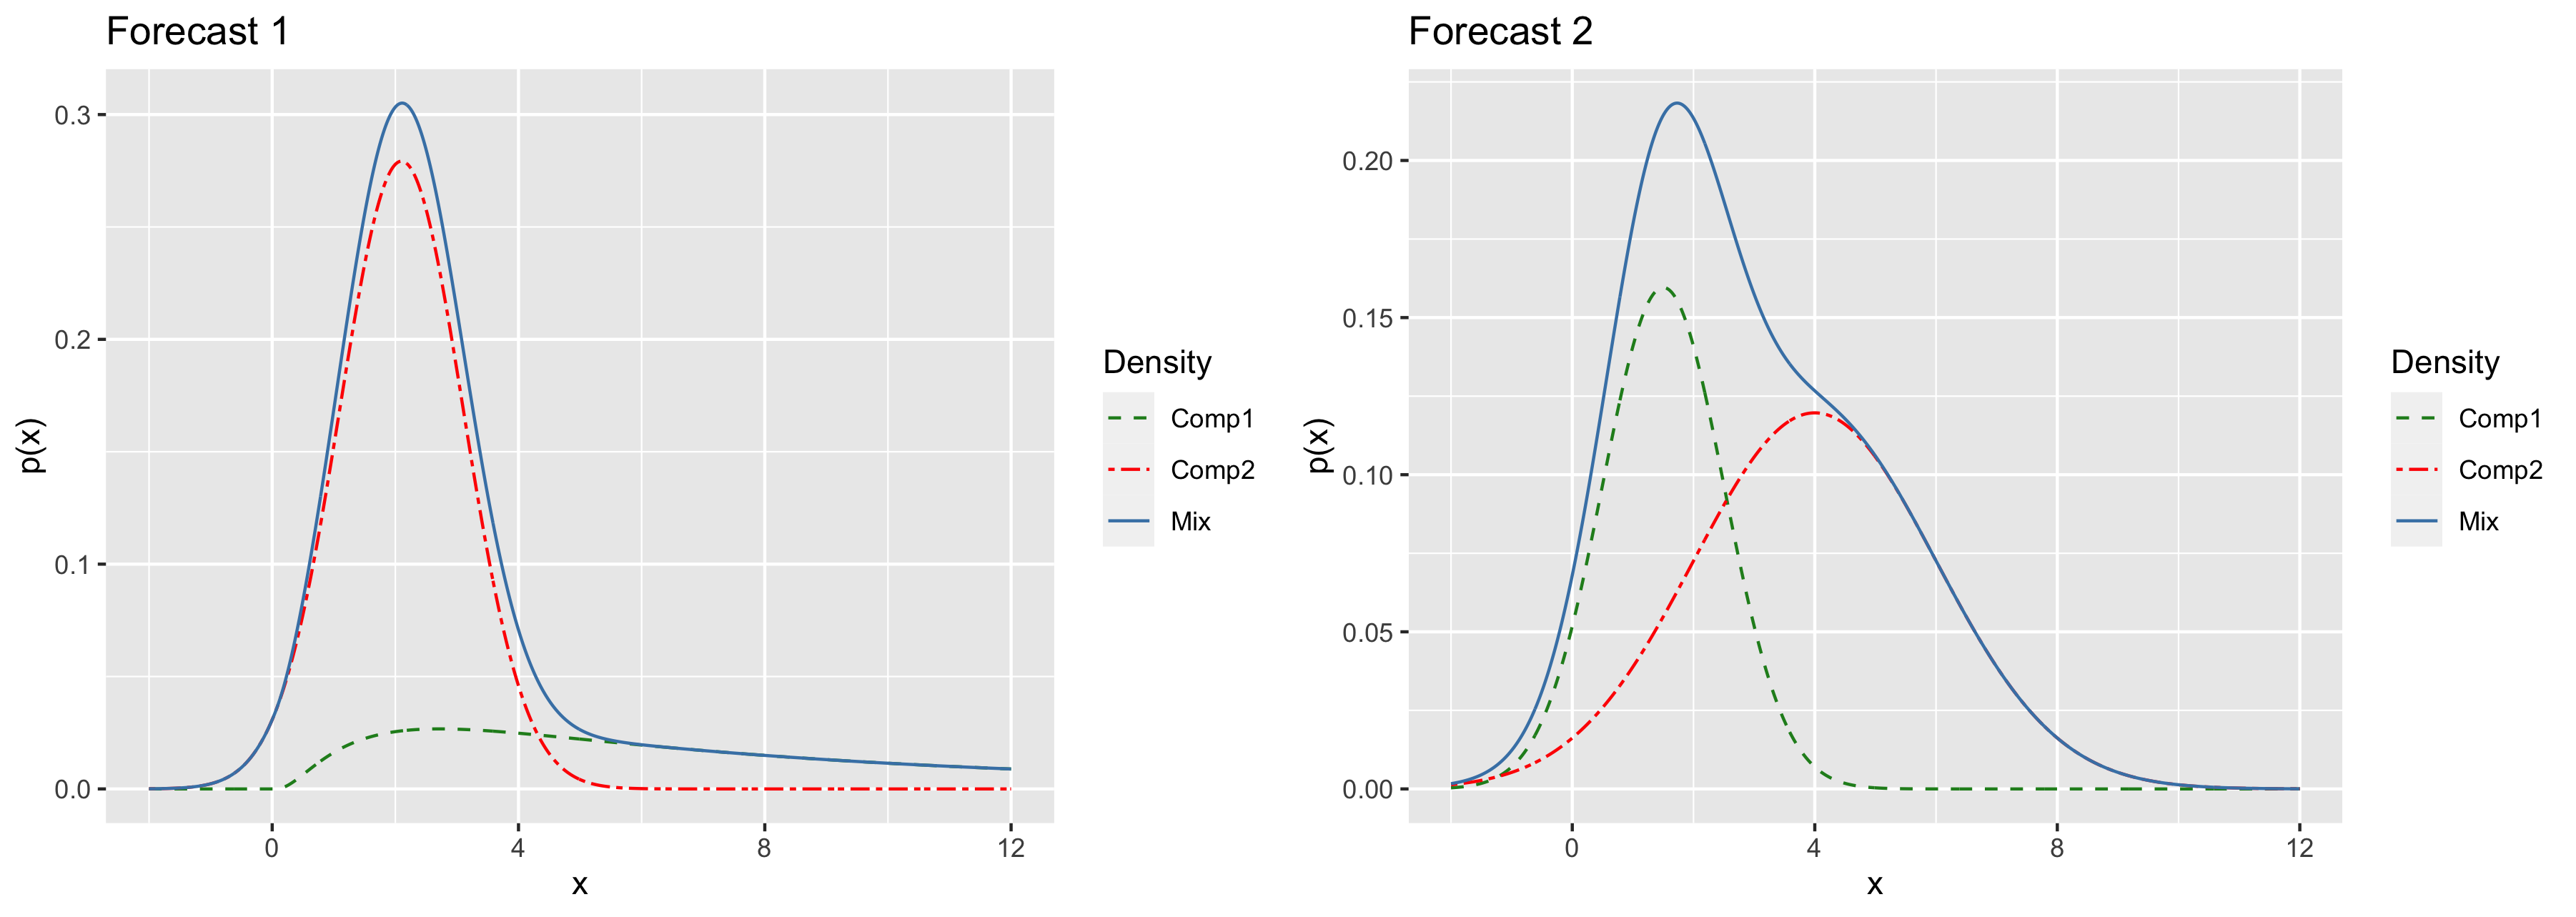
\includegraphics[scale=.15]{Images/toyfors12.png}}
\begin{center}
 \begin{minipage}{11cm}
\captionsetup{font=scriptsize}
\caption[Example mixture distributions]{These plots show the density functions 
of
the two example mixture distribution forecasts along with the component density
functions scaled by the corresponding weights}
\label{fig:toymixs}
\end{minipage}
\end{center}
\end{figure}

Here we include code to illustrate the process of constructing and scoring two 
separate forecasts. We suppose that Table \ref{tab:preddf1} represents a 
submitted forecast from one forecaster and Table \ref{tab:preddf2} represents
a forecast of the same event from a second forecaster. Table \ref{fig:toymixs}
shows plots of the pdfs for both mixture forecasts.
Note the additional \texttt{param3} variable
in Tables \ref{tab:preddf1} and \ref{tab:preddf1}. This variable is included
in the table because of the functionality of the \texttt{MakeDist()} function
which allows for component distributions of up to three parameters.
The code here shows these two forecasts as \texttt{data.frame}s and how the 
\texttt{MakeDist()} 
function is used to create the distributions in \texttt{R}. Once the 
distributions are created as \texttt{AbscontDistribution} objects, then 
functions for evaluating a pdf and a CDF for each are created.







\begin{Schunk}
\begin{Sinput}
> preddf1
\end{Sinput}
\begin{Soutput}
  family param1 param2 param3 weights
1  Lnorm    2.0      1     NA     0.3
2   Norm    2.1      1     NA     0.7
\end{Soutput}
\begin{Sinput}
> preddf2
\end{Sinput}
\begin{Soutput}
  family param1 param2 param3 weights
1   Norm    1.5      1     NA     0.4
2   Norm    4.0      2     NA     0.6
\end{Soutput}
\begin{Sinput}
> #make mixture distributions from prediction submissions
> mdist1 <- MakeDist(preddf1)
> mdist2 <- MakeDist(preddf2)
\end{Sinput}
\end{Schunk}

\begin{Schunk}
\begin{Sinput}
> #make pdfs for mixture predictions
> dmdist1 <- function(x) {distr::d(mdist1)(x)}
> dmdist2 <- function(x) {distr::d(mdist2)(x)}
> #make cdfs for mixture predictions
> pmdist1 <- function(x) {distr::p(mdist1)(x)}
> pmdist2 <- function(x) {distr::p(mdist2)(x)}
\end{Sinput}
\end{Schunk}




The LogS or the CRPS may then be calculated for each forecast using the pdf
and CDF functions respectively. Here will will assume that the realized value
which both forecasts attempted to predict was \texttt{3}. 
The \texttt{CRPS()} function
here is one that we wrote and is
included in the APPENDIX. It is seen in the code below that under the
LogS, forecast 1 from table \ref{tab:preddf1} outperforms forecast 2 from table
\ref{tab:preddf2} with scores of 1.547 and 
1.849 respectively. 
However, under the CRPS forecast 2 outperforms forecast 1
with scores 0.635 and 
0.635 respectively. We continue to use these same
forecasts in Section \ref{section:enscon} to construct an ensemble forecast.

\begin{Schunk}
\begin{Sinput}
> #realized observation
> ob <- 3
> #LogS for predictions at the realized observation
> -log(dmdist1(ob))
\end{Sinput}
\begin{Soutput}
[1] 1.547238
\end{Soutput}
\begin{Sinput}
> -log(dmdist2(ob))
\end{Sinput}
\begin{Soutput}
[1] 1.848796
\end{Soutput}
\end{Schunk}

\begin{Schunk}
\begin{Sinput}
> #CRPS for predictions at the realized observation
> CRPS(pmdist1,y=ob)
\end{Sinput}
\begin{Soutput}
[1] 0.6348212
\end{Soutput}
\begin{Sinput}
> CRPS(pmdist2,y=ob)
\end{Sinput}
\begin{Soutput}
[1] 0.5306083
\end{Soutput}
\end{Schunk}

\section{Ensemble construction}
\label{section:enscon}


To construct an ensemble distribution from multiple mixture distributions, the 
\texttt{UnivarMixingDistribution()} is again a useful tool. The function takes 
two or more
\texttt{AbscontDistribution} distribution objects and a vector of weights 
corresponding to each object. A new \texttt{AbscontDistribution} object is 
returned as an ensemble of mixture distributions as in (\ref{eq:bma}). 
Since they are \texttt{AbscontDistribution} objects \texttt{mdist1} and 
\texttt{mdist2} created in the code
in Section \ref{section:tools} may be input as arguments into the function
\texttt{UnivarMixingDistribution()}, but weights for each object need to also
be determined.

At the onset of a collaborative forecast before there are true event 
observations which the forecasts can be scored on, 
it may make sense to assign an equal weight to each 
component distribution in an ensemble. As a project progresses however, 
assigning weights based on past performance may be desired. As mentioned in 
section \ref{section:pardist}, weights may be selected by maximizing the
likelihood of (\ref{eq:bma}) or by minimizing the CRPS. Another method of 
selecting weights is to use the posterior model probability. 

If we have $T$ models ($M_t$) the posterior model probability of $M_t$ is 
defined as in \eqref{eq:pmp} where $p(\cdot |M_t) := p_m(\cdot)$ is the density 
function of the model and 
$p(M_j)$ is the prior probability assigned to the model. A common approach is to
assume the prior
probabilities for each model are equal or $p(M_t) = 1/T$ for all $t$ in which 
case
(\ref{eq:pmp}) is reduced to \eqref{eq:pmpeq}. In this case the posterior model 
probability for model $t$ is equal to the exponential of its negative LogS or
$p(M_t|x) = e^{-LogS(p(M_t|x))}$, so the performance of a forecast based on the
LogS is directly related to posterior model probability and may be used as an 
ensemble weight. For an observed event $x^*$, ensemble weights $(w_t)$ from 
\eqref{eq:bma} may be defined as $w_t := p(M_t|x^*)$.


\begin{equation}
\label{eq:pmp}
p(M_t|x) = \frac{p(x|M_t)p(M_t)}{p(x)}
         = \frac{p(x|M_t)p(M_t)}{\sum_{k=1}^T p(x|M_k)p(M_k)}
\end{equation}


\begin{equation}
\label{eq:pmpeq}
p(M_t|x) =  \frac{p(x|M_t)}{\sum_{k=1}^Tp(x|M_k)}
\end{equation}



Using the illustrative example from Section \ref{section:tools}, 
the following code shows how
to use the posterior model probability to select weights and construct an 
ensemble distribution and score the ensemble forecast. Here again we take the 
observed value to be \texttt{3}.
The ensemble distribution
with components is show in figure \ref{fig:mixense}.

\begin{Schunk}
\begin{Sinput}
> #posterior model probability for calculating weights
> w1 <- pmdist1(ob)/(pmdist1(ob) + pmdist2(ob))
> w2 <- 1-w1
> w1
\end{Sinput}
\begin{Soutput}
[1] 0.5286434
\end{Soutput}
\begin{Sinput}
> w2
\end{Sinput}
\begin{Soutput}
[1] 0.4713566
\end{Soutput}
\begin{Sinput}
> #build ensemble with calculated weights
> ensdist <- distr::UnivarMixingDistribution(mdist1,
+                                            mdist2,
+                                            mixCoeff = c(w1,w2))
> #pdf and cdf for ensemble
> densdist <- function(x) {(distr::d(ensdist)(x))}
> pensdist <- function(x) {(distr::p(ensdist)(x))}
> #LogS for predictions at the realized observation
> -log(densdist(ob))
\end{Sinput}
\begin{Soutput}
[1] 1.678156
\end{Soutput}
\begin{Sinput}
> #CRPS for predictions at the realized observation
> CRPS(pensdist,y=ob)
\end{Sinput}
\begin{Soutput}
[1] 0.5486368
\end{Soutput}
\end{Schunk}


\begin{figure}[htbp]
\centerline{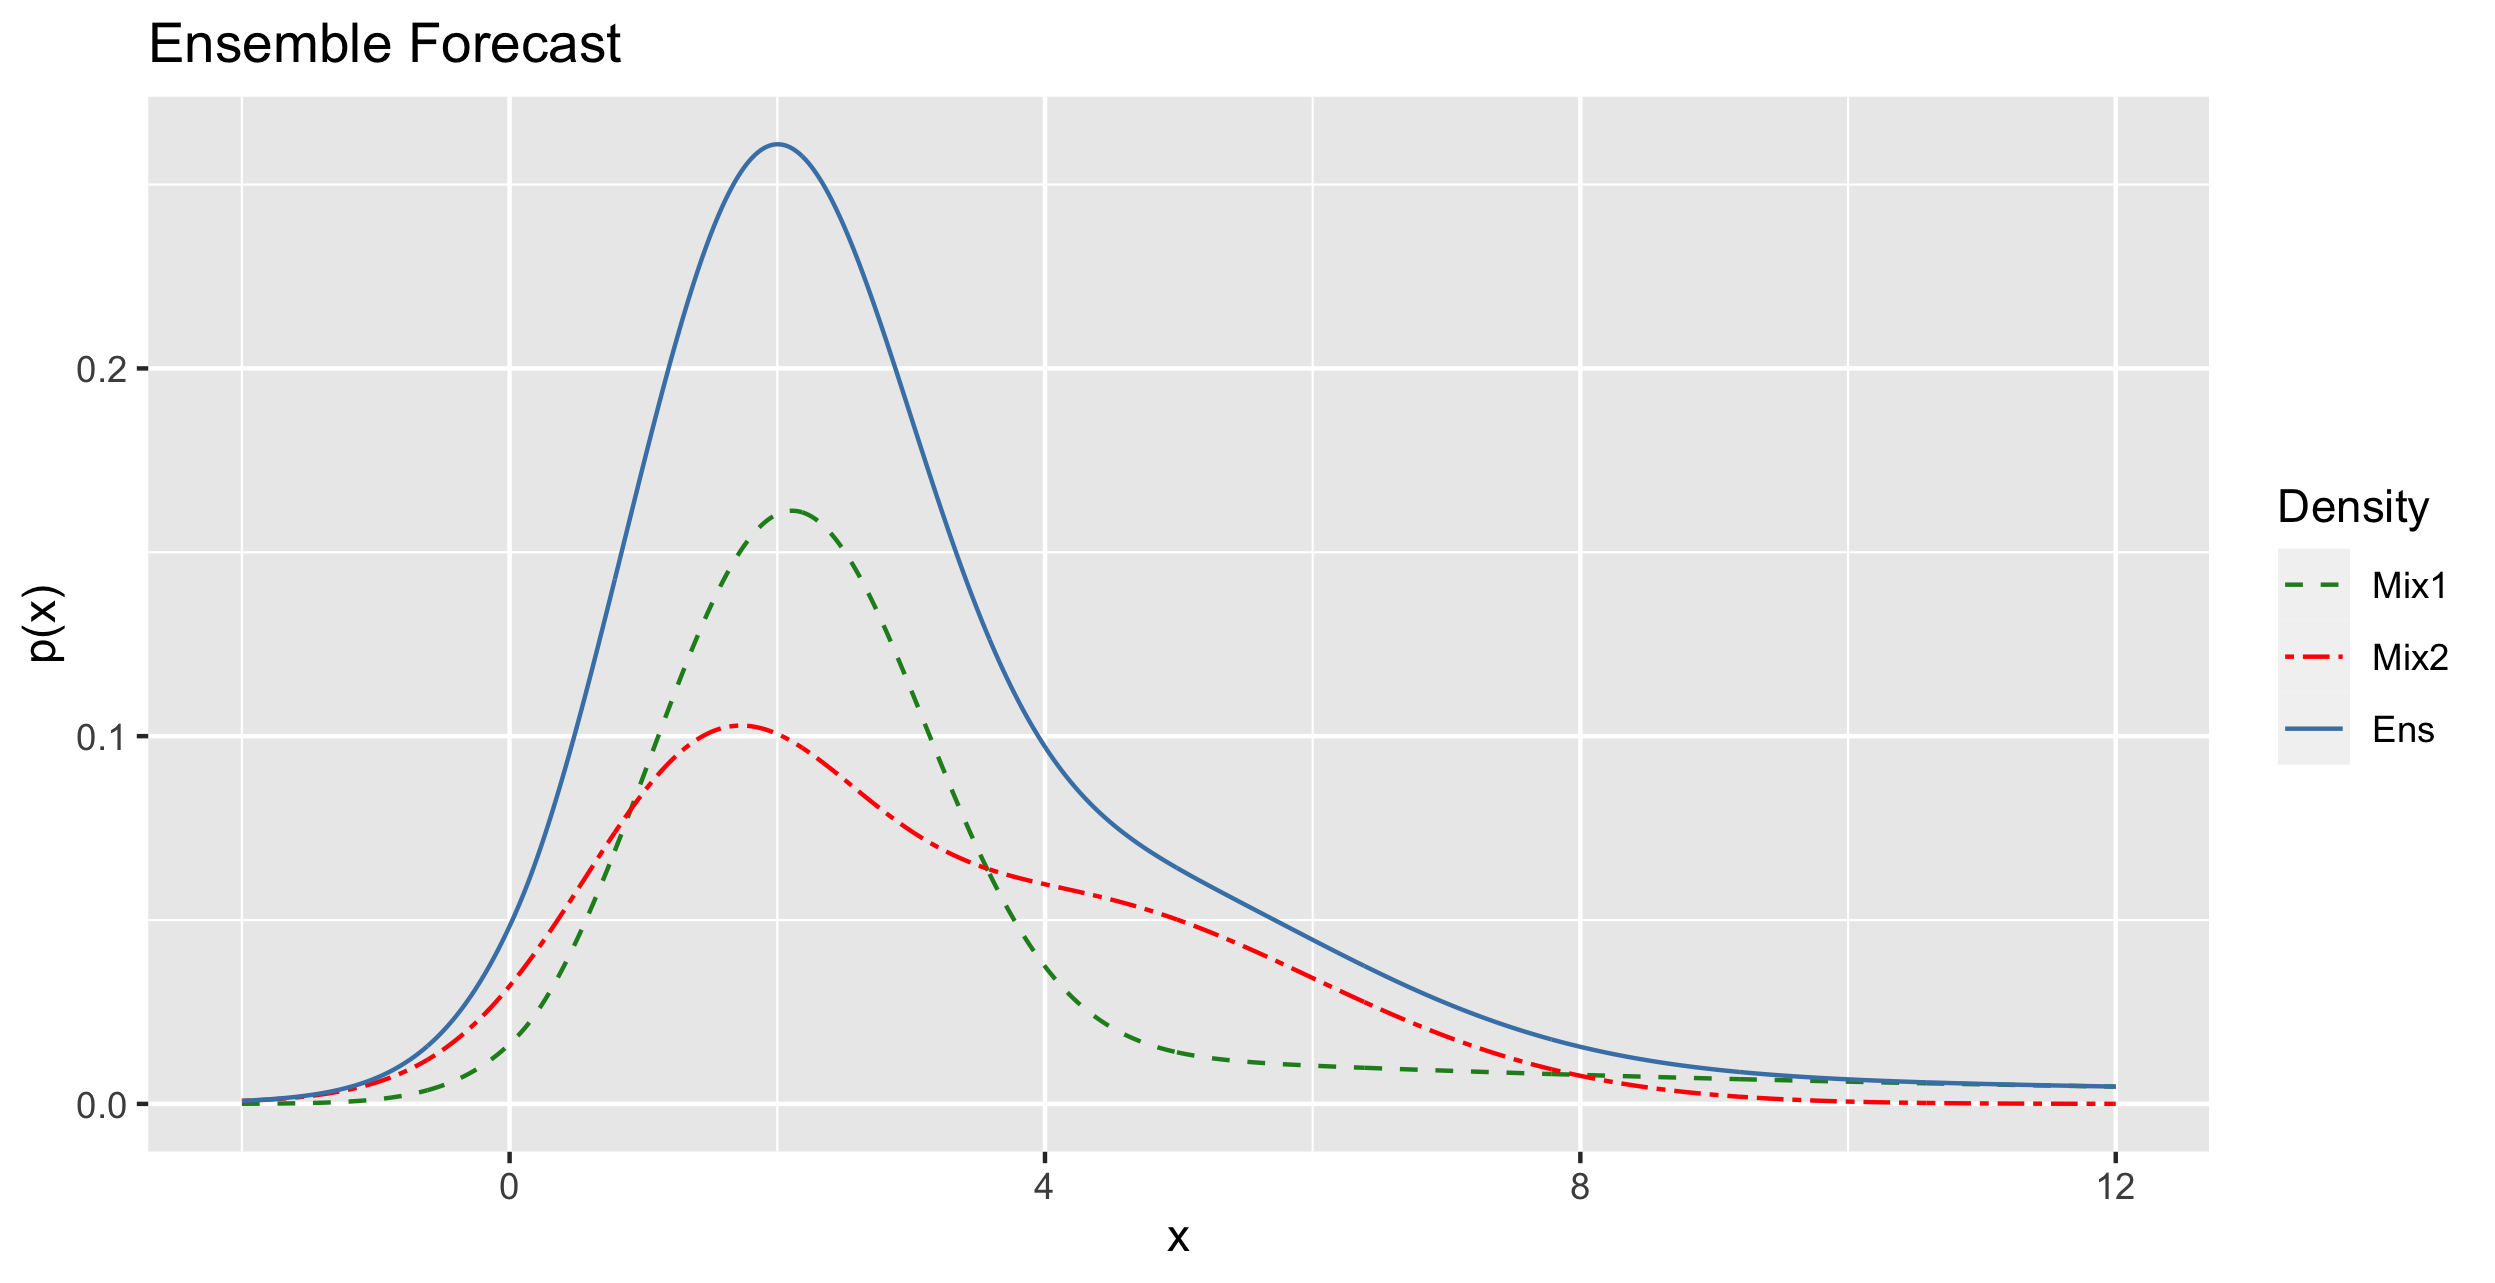
\includegraphics[scale=.15]{Images/mix_ense.png}}
\caption[Example ensemble forecast]{Ensemble forecast made from forecast 1 and 
forecast 2 from Section \ref{section:tools}. The green line is the density 
component of mixture forecast 1 with weight 0.529. The 
red line is the density component of mixture forecast 2 with weight 
0.471. The blue line is the density of the ensemble.}
\label{fig:mixense}
\end{figure}

% \subsection{Mixture approximation of sample distribution}





















\chapter{Retrospective analysis}
\label{section:retrostud}

For large collaborative forecast projects having already established the 
representation formats for forecasting, it may be difficult for individual
forecast teams to adjust to a mixture distribution format. There may be several
reasons for this, including that not all 
forecast modeling methods will produce forecasts which may conveniently be
represented by a mixture distribution.
In this section we attempt to assess whether or not any forecasts from the CDC
flu competition and the COVID-19 Forecast Hub were generated from one component
mixture distribution models. We do this by fitting one component mixture 
distributions to the forecasts and assessing how well the fit models represent
the forecasts.

Forecasters in both the CDC flu competition and the COVID-19 Forecast Hub do 
not include with their forecast submissions information about modeling methods 
or 
distributional assumptions. Thus the only information we have for fitting
distributions are bin
forecasts and quantile forecasts. We are unaware of formal statistical 
methods for fitting parametric distributions or mixture distributions to bin
distributions. Methods of fitting a distribution to quantiles 
include Bayesian Quantile Matching
\cite[]{nirwan2020bayesian}, step interpolation with exponential tails 
\cite[]{quinonero2005evaluating},
and the Method of Simulated Quantiles 
\cite[]{dominicy2013method}. These studies however lack claims that the methods
for fitting are statistically formal.
Because of this it should be noted that any conclusions made in 
this section may not be 
stated in terms of statistical certainty.



\section{CDC flu competition}
The CDC Retrospective Forecasts project on zoltrdata.com \cite[]{zoltarflu} 
contains over
869,638 probabilistic influenza-like illness forecasts for all combinations
of 11 regions 
in the United States and seven targets from 27 different modeling teams. These
include forecasts made during all flu seasons between October 2010 and December
2018. All forecasts are represented by bin distributions. 
We wanted to determine whether or not any of these forecasts were
generated from one component mixture distributions of continuous uniform, 
truncated normal (TN), truncated
lognormal (TL), or truncated gamma (TG) distribution families.
The process we followed for determining if a forecast was generated by one of
these common families was to first fit a distribution of that family to the bin
forecast and then measure close the fit was. The decsion to fit truncated 
distributions was due to all bin forecasts being assessed having a finite 
support.

To fit a distribution to a forecast we first minimize \eqref{eq:msd}. We call
\eqref{eq:msd} the mean square difference (MSD).
Here $F(\cdot| \hat{\theta})$ is a CDF, $p_i$ is the reported probability for 
the $i^{th}$ bin $B_i := [b_{i-1}, b_i)$ and $K$ is the number of bins.
The fitted parameter vector $\hat{\theta}$ is the solution to 
\eqref{eq:discfit}.
If a distribution was fit to the submitted binned 
prediction
and the MSD was less than a 
specified cutoff value, we
concluded that the bin forecast may have been discretized from the 
distribution.

\begin{equation}
  MSD = \sum_{i=1}^K (p_i - [F(b_i| \hat{\theta}) - F(b_{i-1}| \hat{\theta})])^2
  \label{eq:msd}
\end{equation}


\begin{equation}
\hat{\theta} = \arg\min_{\theta}\sum_{i=1}^K (p_i - 
[F(b_i; \theta) - F(b_{i-1}; \theta)])^2
\label{eq:discfit}
\end{equation}




To determine what values to use as cutoffs we conducted a study where 
bin distributions were discretized from known distributions, 
parameters were fit to the binned distrubtions and the MSD was calculated. This 
was done 1,000 times for the four distrubtion families considered and the cutoff 
value for each family was set as the value under which 95\% of MSD values fell.
The exact process is as follows.

For each of uniform, TN, TL, and 
TG distributions the following was
done 1,000 times. A set of 131 bins with interval widths of 
0.1 between 0 and 13 was constructed. 
A value $u$ was selected from a $\mbox{Unif(0,13)}$ distribution and $y$ from 
a $\mbox{Unif(.05,1.6)}$ distribution. 
$u$ and $y$ were taken as respectively 
the center and scale parameters of a TN distribution. 
For uniform, TL, and TG family
distributions, model parameters were solved for so that $u$ and $y$ 
were roughly the mean and standard deviation.
% Had we accounted for the changes
% in moment values from the truncation, the means and standard deviations could 
% have been exactly $\mu$ and $\sigma$. But we considered the differences small 
% enough that it didn't matter for our purpose.
With a known distribution with $\theta = (u,y)$, 
probabilities $p_i =F(b_i| \theta) - F(b_{i-1})$ 
where, were
calculated for each bin. A distribution from the same
family was fit to the bins by minimizing \eqref{eq:msd} with the resulting
distribution function $F(\cdot| \hat{\theta})$. 
The minimization was done using 
the \texttt{optim} function in the \texttt{R} \texttt{stats} package.
From the fit distribution
$\hat{p_i} = F(b_i; \hat{\theta}) - F(b_{i-1}; \hat{\theta})$ was computed for 
each of the 131 bins. Finally the MSD was calculated. 
Table \ref{table:bincutoffs}
below shows MSD value for which 95\% of all 1,000 MSDs fell below. Those values 
were selected as the 
cutoff values for declaring whether or not a bin distribution was discretized
from from a one component mixture distribution of that family.


\begin{table}[h!]
  \centering
  \begin{tabular}{l*{6}{c}r}
  Distribution          & MSD 95\% Cutoff \\
  \hline
  Uniform               & 8.809460e-05   \\
  Truncated Normal      & 1.126683e-07  \\
  Truncated Lognormal   & 3.877829e-06  \\
  Truncated Gamma       & 1.500152e-06  \\
  \end{tabular}
  \begin{center}
\begin{minipage}{10cm}
\captionsetup{font=scriptsize}
  \caption[Bin distribution cutoff values]{If a binned 
  one component mixture distribution is fit to a bin forecast
  and the MSD is smaller than
  the corresponding cutoff value listed here, we consider that bin 
  distribution to have been discretized from the fit mixture distribution.}
  \label{table:bincutoffs}
  \end{minipage}
  \end{center}
\end{table}




Of the 869,638 predictions from the CDC Retrospective Forecast project, we fit
each of uniform, TN, TL, and TG distributions to 11,715 of the individual 
predictions. From each of the 27 teams represented, there is a list of forecast
submissions from which we randomly selected 12. From each submission, we 
we randomly selected six forecasts.
In many cases the \texttt{optim} function used to fit the 
distributions failed to converge, so of all forecasts we were only able to 
successfully fit distributions to 11,715 of them.
We calculated the MSD, and for each forecast the fit
distribution with the lowest of the four MSDs was considered the best fit. If 
the MSD from the best fit fell
below the corresponding cutoff value listed in \ref{table:bincutoffs} we 
concluded that 
the forecast was discretized from the fit distribution. 

Table \ref{table:bincutoffs} shows the results of this analysis. 
Of the 11,715 binned distributions fit to the mixture distributions,
2,502 of those fits had MSD values below the values listed in Table
\ref{table:bincutoffs}. Thus we conclude that a proportion of 0.214 of those
forecasts were generated from a common parametric distribution. The results for 
the
11,715 fit distributions, which families the binned distributions were best
fit to and whether or not the fits produce an MSD below the cutoff value, 
are seen in table \ref{table:cdcresults}. Figure \ref{fig:binparamfits} is an
example of
the fit distributions to the same bin forecast.

\begin{table}[h!]
  \centering
  \begin{tabular}{l*{6}{c}r}
  Distribution Family   & Total    & Total below MSD cutoff value 
  & Proportion from parametric distribution\\
  \hline
  Uniform               & 896      & 669  & 0.747  \\
  Truncated Normal      & 3,804    & 198  & 0.052  \\
  Truncated Lognormal   & 4,501    & 1,340 & 0.289 \\
  Truncated Gamma       & 2,514    & 295   & 0.117 \\
  \end{tabular}
  \begin{center}
\begin{minipage}{10cm}
\captionsetup{font=scriptsize}
  \caption[CDC flu retro analysis results]{Of the 11,715
forecasts 864 were best fit by a uniform distribution, 3,804 by a TN, 
4,501 by a TL, and 2,514 by a TG. Of those forecasts, 669 appear to have
come from a uniform distribution, 198 from a TN, 1,340 from a TL, and 295 from
a TG.
}
  \label{table:cdcresults}
  \end{minipage}
  \end{center}
\end{table}

\begin{figure}[htbp]
\centerline{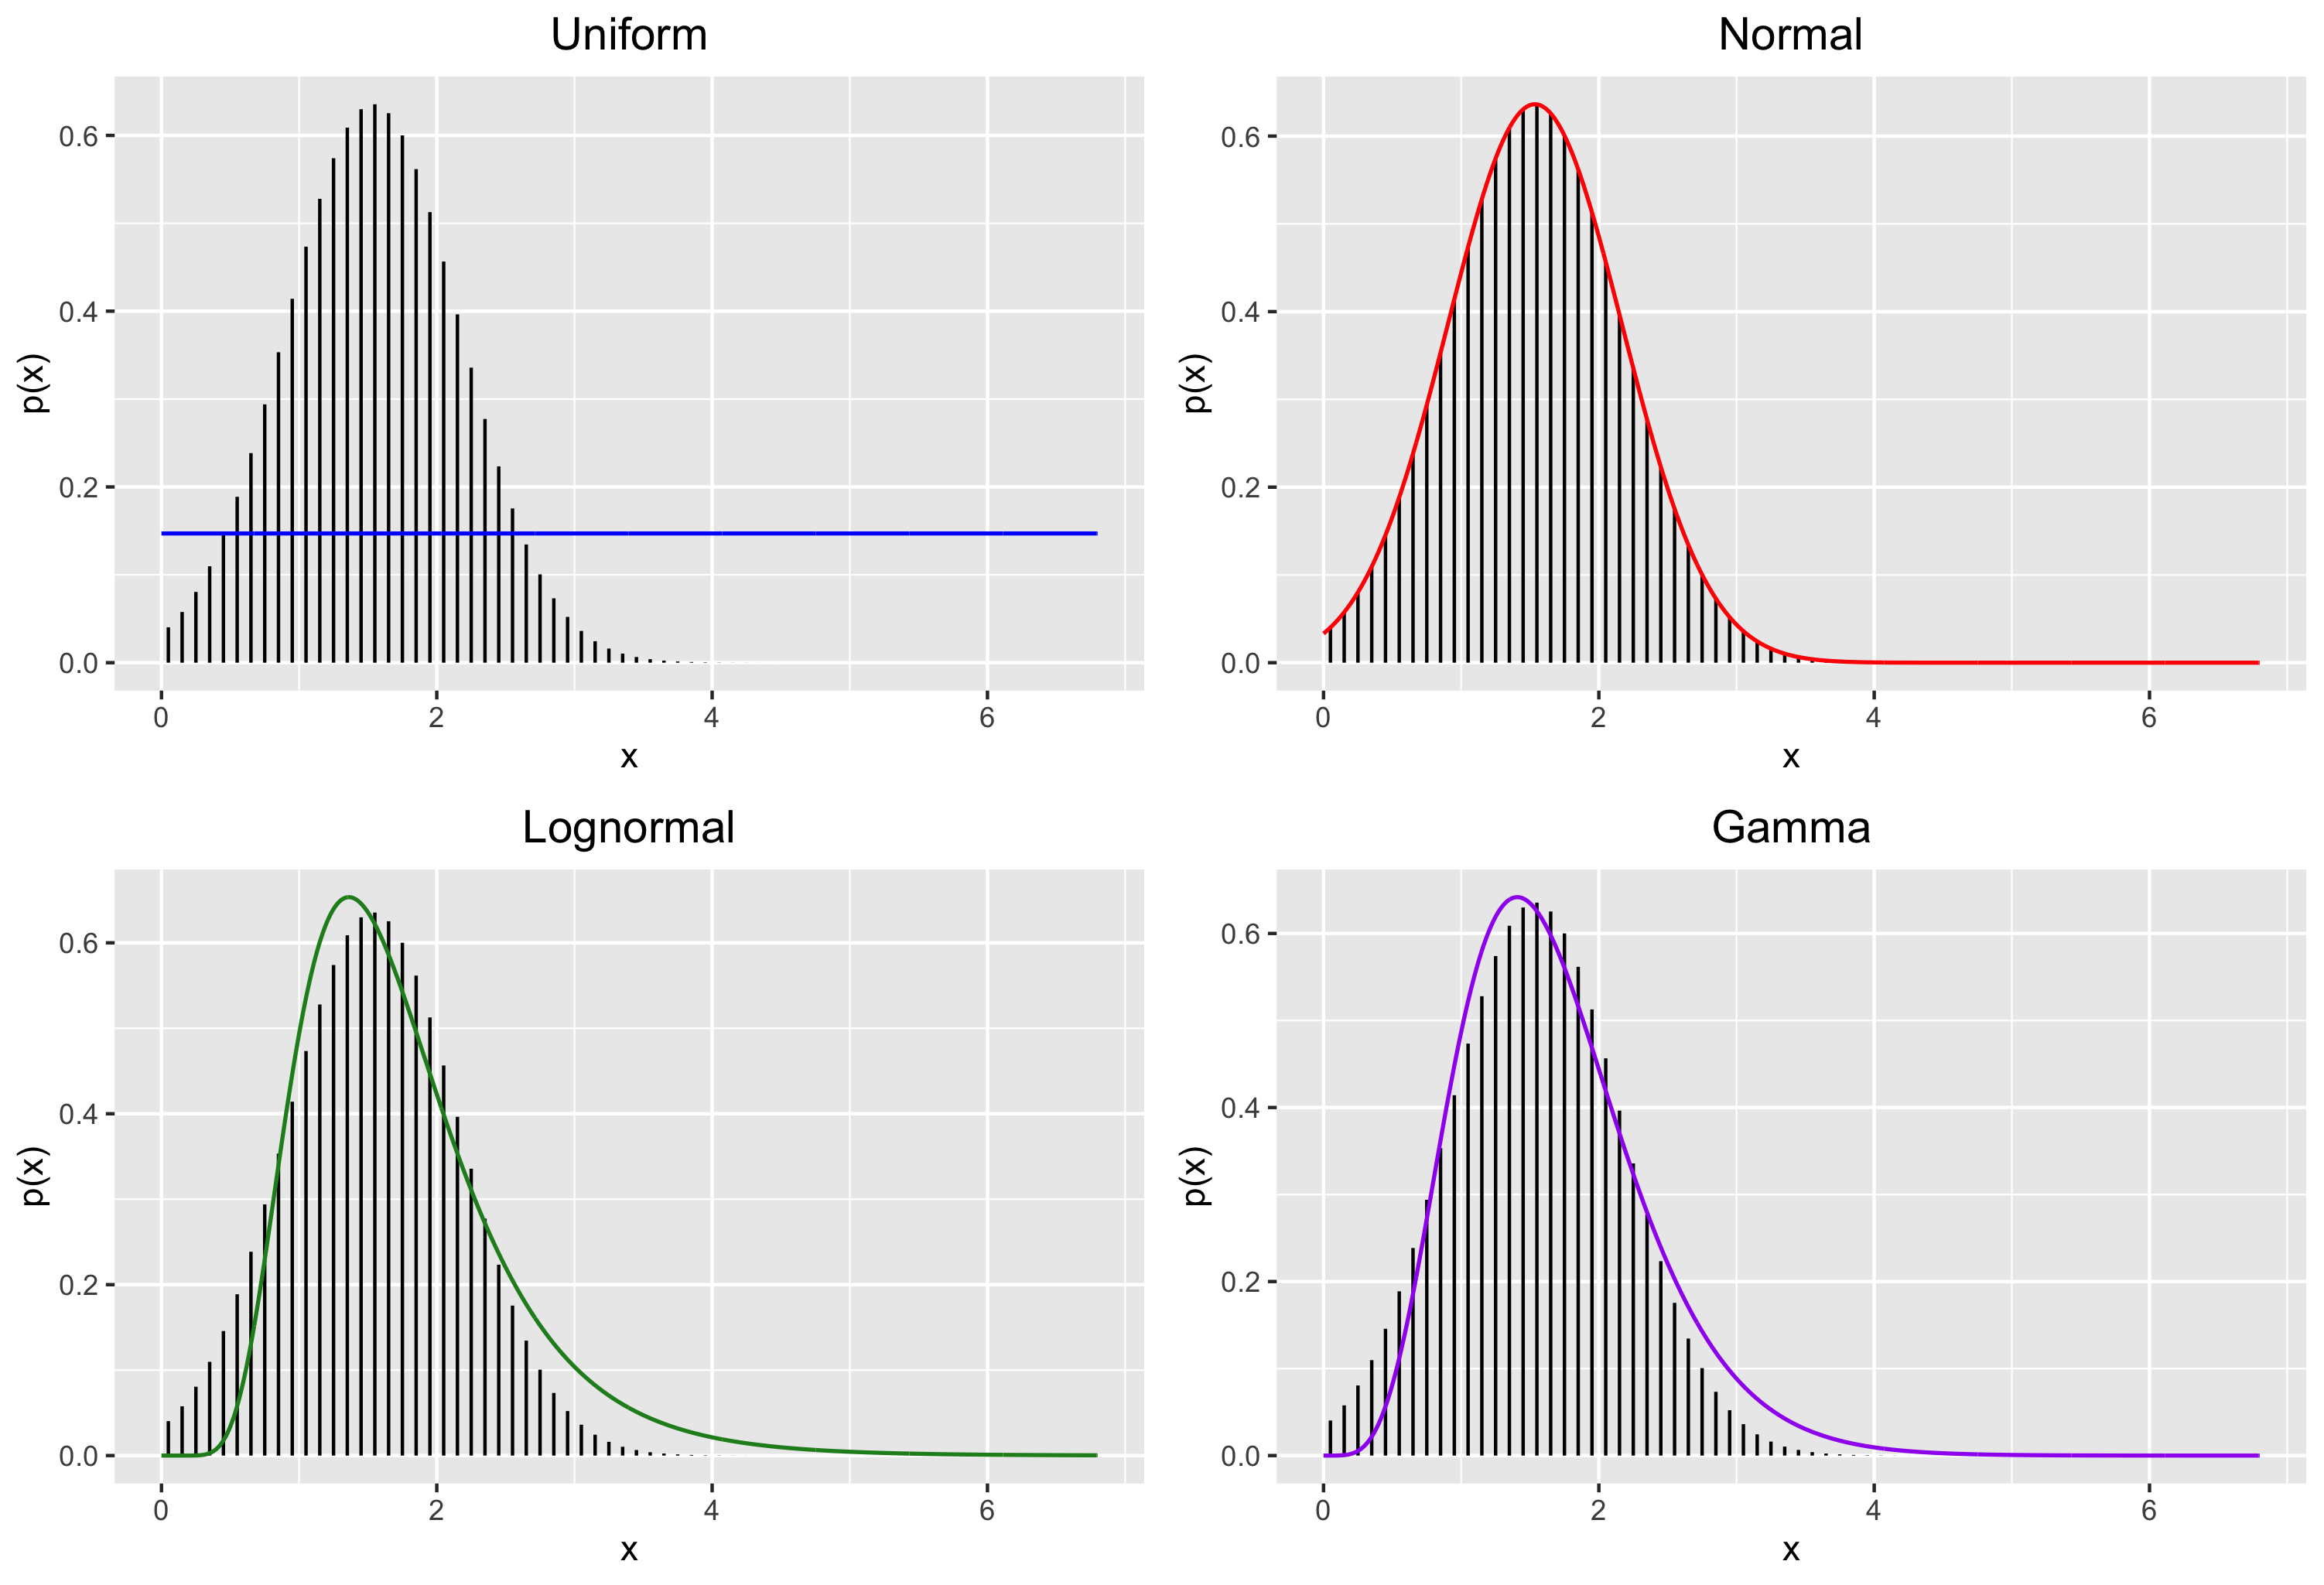
\includegraphics[scale=.15]{Images/flu_fit_17_10_3.png}}
\begin{center}
\begin{minipage}{10cm}
\captionsetup{font=scriptsize}
\caption[Parametric distribution fits to binned distribution]{This figure shows
the plots of fits from each a uniform, TN, TL,
and TG distributions to the same bin distribution. Each black vertical line is
a bin probability $p_i \times 10$. The probabilities are multiplied by 10 to 
better illustrate fitting a distribution to the probabilities.
The title of this forecast
given by the submission team is Bayesian Model Averaging. This forecast was
submitted to the CDC on May 15, 2017 and is a three week ahead forecast of
percent of hospital patients due to an influenza like illness for a specific
region of the United States.
In this case, the fit to the normal distribution produced an MSD below the 
TN cutoff value, so we conclude that the bin forecast may have been
discretized from a TN. Proportions of distributions with MSDs 
below the cutoff values are also included.}
\label{fig:binparamfits}
\end{minipage}
\end{center}
\end{figure}



\section{COVID-19 Forecast Hub}

As of April 4, 2022 there were over 90 million forecasts  
from 117 different modeling teams submitted to the COVID-19 Forecast Hub 
\cite[]{zoltarcovid}. 
These 
forecasts covered all combinations of 3,202 municipalities (mostly counties) 
in the United States with 441 targets. The first of these forecasts was 
submitted in March of 2020 shortly after the initial outbreak of the COVID-19 
virus in 
the US and forecasts have been received weekly since. 
The forecasts are all quantile forecasts made up of three or 11 predictive 
intervals -depending on the specific unit for the forecast-
and a median. In the forecasts include seven or 23 quantiles.

To assess whether or not a quantile forecast was calculated from a well
known continuous distribution, we minimized the mean square error (MSE)  
in \eqref{eq:mse} between where $q_i$ is
the $i^{th}$ quantile value from a forecast and $F(y| \theta)$ is a fit CDF with 
parameter $\hat{\theta}$. The parameter $\hat{\theta}$ is the solution to 
\eqref{eq:minthet}.

\begin{equation}
  MSE = \sum_{i=1}^m (q_i - F(y| \hat{\theta}))
  \label{eq:mse}
\end{equation}

\begin{equation}
  \hat{\theta} = \arg\min_{\theta} \sum_{i=1}^m (q_i - F(y| \theta))
  \label{eq:minthet}
\end{equation}




For each forecast assessed, we fit the quantiles to a uniform, normal, 
lognormal,
gamma, and location-scale t CDF. Unlike in the previous section, we felt no need
to the distributions as truncated because there is no range limit to these 
forecasts. We included the t distribution to account for any
symmetric forecasts with heavier tails than in a normal distribution.
If the MSE between a given forecast and a fit CDF fell below a certain cutoff,
we considered the quantiles as approximately coming from the fit CDF. To
determine the cutoff values, for each of the five distribution families the same
procedure was followed 1,000 times. 

A decision was randomly made on creating a quantile distribution with seven 
quantiles or 23
quantiles with probabilities 1/3 and 2/3 respectively. This was done because 
in the COVID-19 Forecast Hub certain target/unit combinations require 
seven quantiles and others 
require 23. After that decision was made, a random value $u$ was drawn from
a $\mbox{Unif(2,000,\; 25,000)}$ distribution and another value $v$ was drawn
from a $\mbox{Unif(3, 200)}$ distribution. These values were taken as the mean 
and
standard deviation and for each of the distribution families considered. The
proper transformations computed to find model parameters corresponding to the 
distribution. Quantile values were calculated for then each quantile. When using 
a t distribution, a value for degrees of freedom was drawn from a 
$\mbox{Unif(2,35)}$ distribution. A CDF
was fit by minimizing \eqref{eq:minthet} over the parameter
vector $\theta$ and the MSE value from \eqref{eq:mse} was 
calculated. The MSE value for which 95\% of the 1,000 simulated distributions
fell below was considered the cutoff for that family and is seen in table 
\ref{table:quantcutoffs}. It is immediately noticeable that the cutoff value 
for the location-scale t family is several orders of magnitude higher than for 
the other distribution families. We believe this is related to the fact that 
that is a three parameter family where as the other four families are two 
parameter families. Thus influencing the optimization methods used enough to 
make such a difference in the cutoff value. 

\begin{table}[h!]
  \centering
  \begin{tabular}{l*{6}{c}r}
  Distribution          & MSE 95\% Cutoff \\
  \hline
  Uniform               & 7.220667e-07   \\
  Normal                & 3.097645e-05  \\
  Lognormal             & 1.166775e-07  \\
  Gamma                 & 2.953370e-05  \\
  Location-scale T      & 0.4894471 \\
  \end{tabular}
  \begin{center}
\begin{minipage}{10cm}
\captionsetup{font=scriptsize}
  \caption[Quantile cutoff values]{If a one component mixture distribution of a
  certain distribution family
  is fit to a quantile forecast and the MSE is smaller than
  the corresponding cutoff value listed here, we conclude the quantiles to 
  have been calculated from the fit distribution.}
  \label{table:quantcutoffs}
  \end{minipage}
  \end{center}
\end{table}


With these cutoff values selected, distributions were then fit to quantile 
forecasts
from the COVID-19 Forecasts on zoltardata.com \cite[]{zoltarcovid}.
From 115 modeling teams we randomly selected four forecast submissions. From 
those submissions we randomly selected three units and attempted to assess
forecasts for all targets under than unit.
This was a computationally more
difficult problem than fitting distributions to the bin forecasts from the CDC
flu competition, so the number of forecasts where convergence for fitting was
met was much smaller. In total distributions from all five families of interest
were fit to 2,504 forecasts. 
The MSE was calculated for each and the fit with the
lowest MSE was selected as the closest fit. If the MSE fell below the cutoff
specified above, we concluded that the quantile forecast was approximately
from the same distribution as the fit distribution. 

Table \ref{table:cresults} show the results of the analysis by distribution
family.
Of the 2,504 fits, 99 of 
them had an MSE value below the corresponding cutoff listed in Table
\ref{table:quantcutoffs}. Thus we conclude that a proportion of 0.04 of the 
forecasts assessed came from distributions fit to them.
Results for fits by
distribution are seen in Table \ref{table:cresults}.
Figures \ref{fig:qqfits} and \ref{fig:cdffits} show the QQ plots and CDF plots
for different distribution fits to the same set of quantiles.



\begin{table}[h!]
  \centering
  \begin{tabular}{l*{6}{c}r}
  Distribution Family   & Total    & Total below MSE cutoff 
  & Proportion from parametric distribution\\
  \hline
  Uniform               & 239      & 0    & 0    \\
  Normal                & 609      & 74   & 0.122    \\
  Lognormal             & 694      & 0    & 0    \\
  Gamma                 & 597      & 0    & 0    \\
  Location-scale T      & 365      & 25   & 0.068    \\
  \end{tabular}
  \begin{center}
\begin{minipage}{10cm}
\captionsetup{font=scriptsize}
  \caption[COVID-19 Forecast Hub results]{Results for COVID-19 Forecast Hub
  retro analysis}
  \label{table:cresults}
  \end{minipage}
  \end{center}
\end{table}


\begin{figure}[htbp]
\centerline{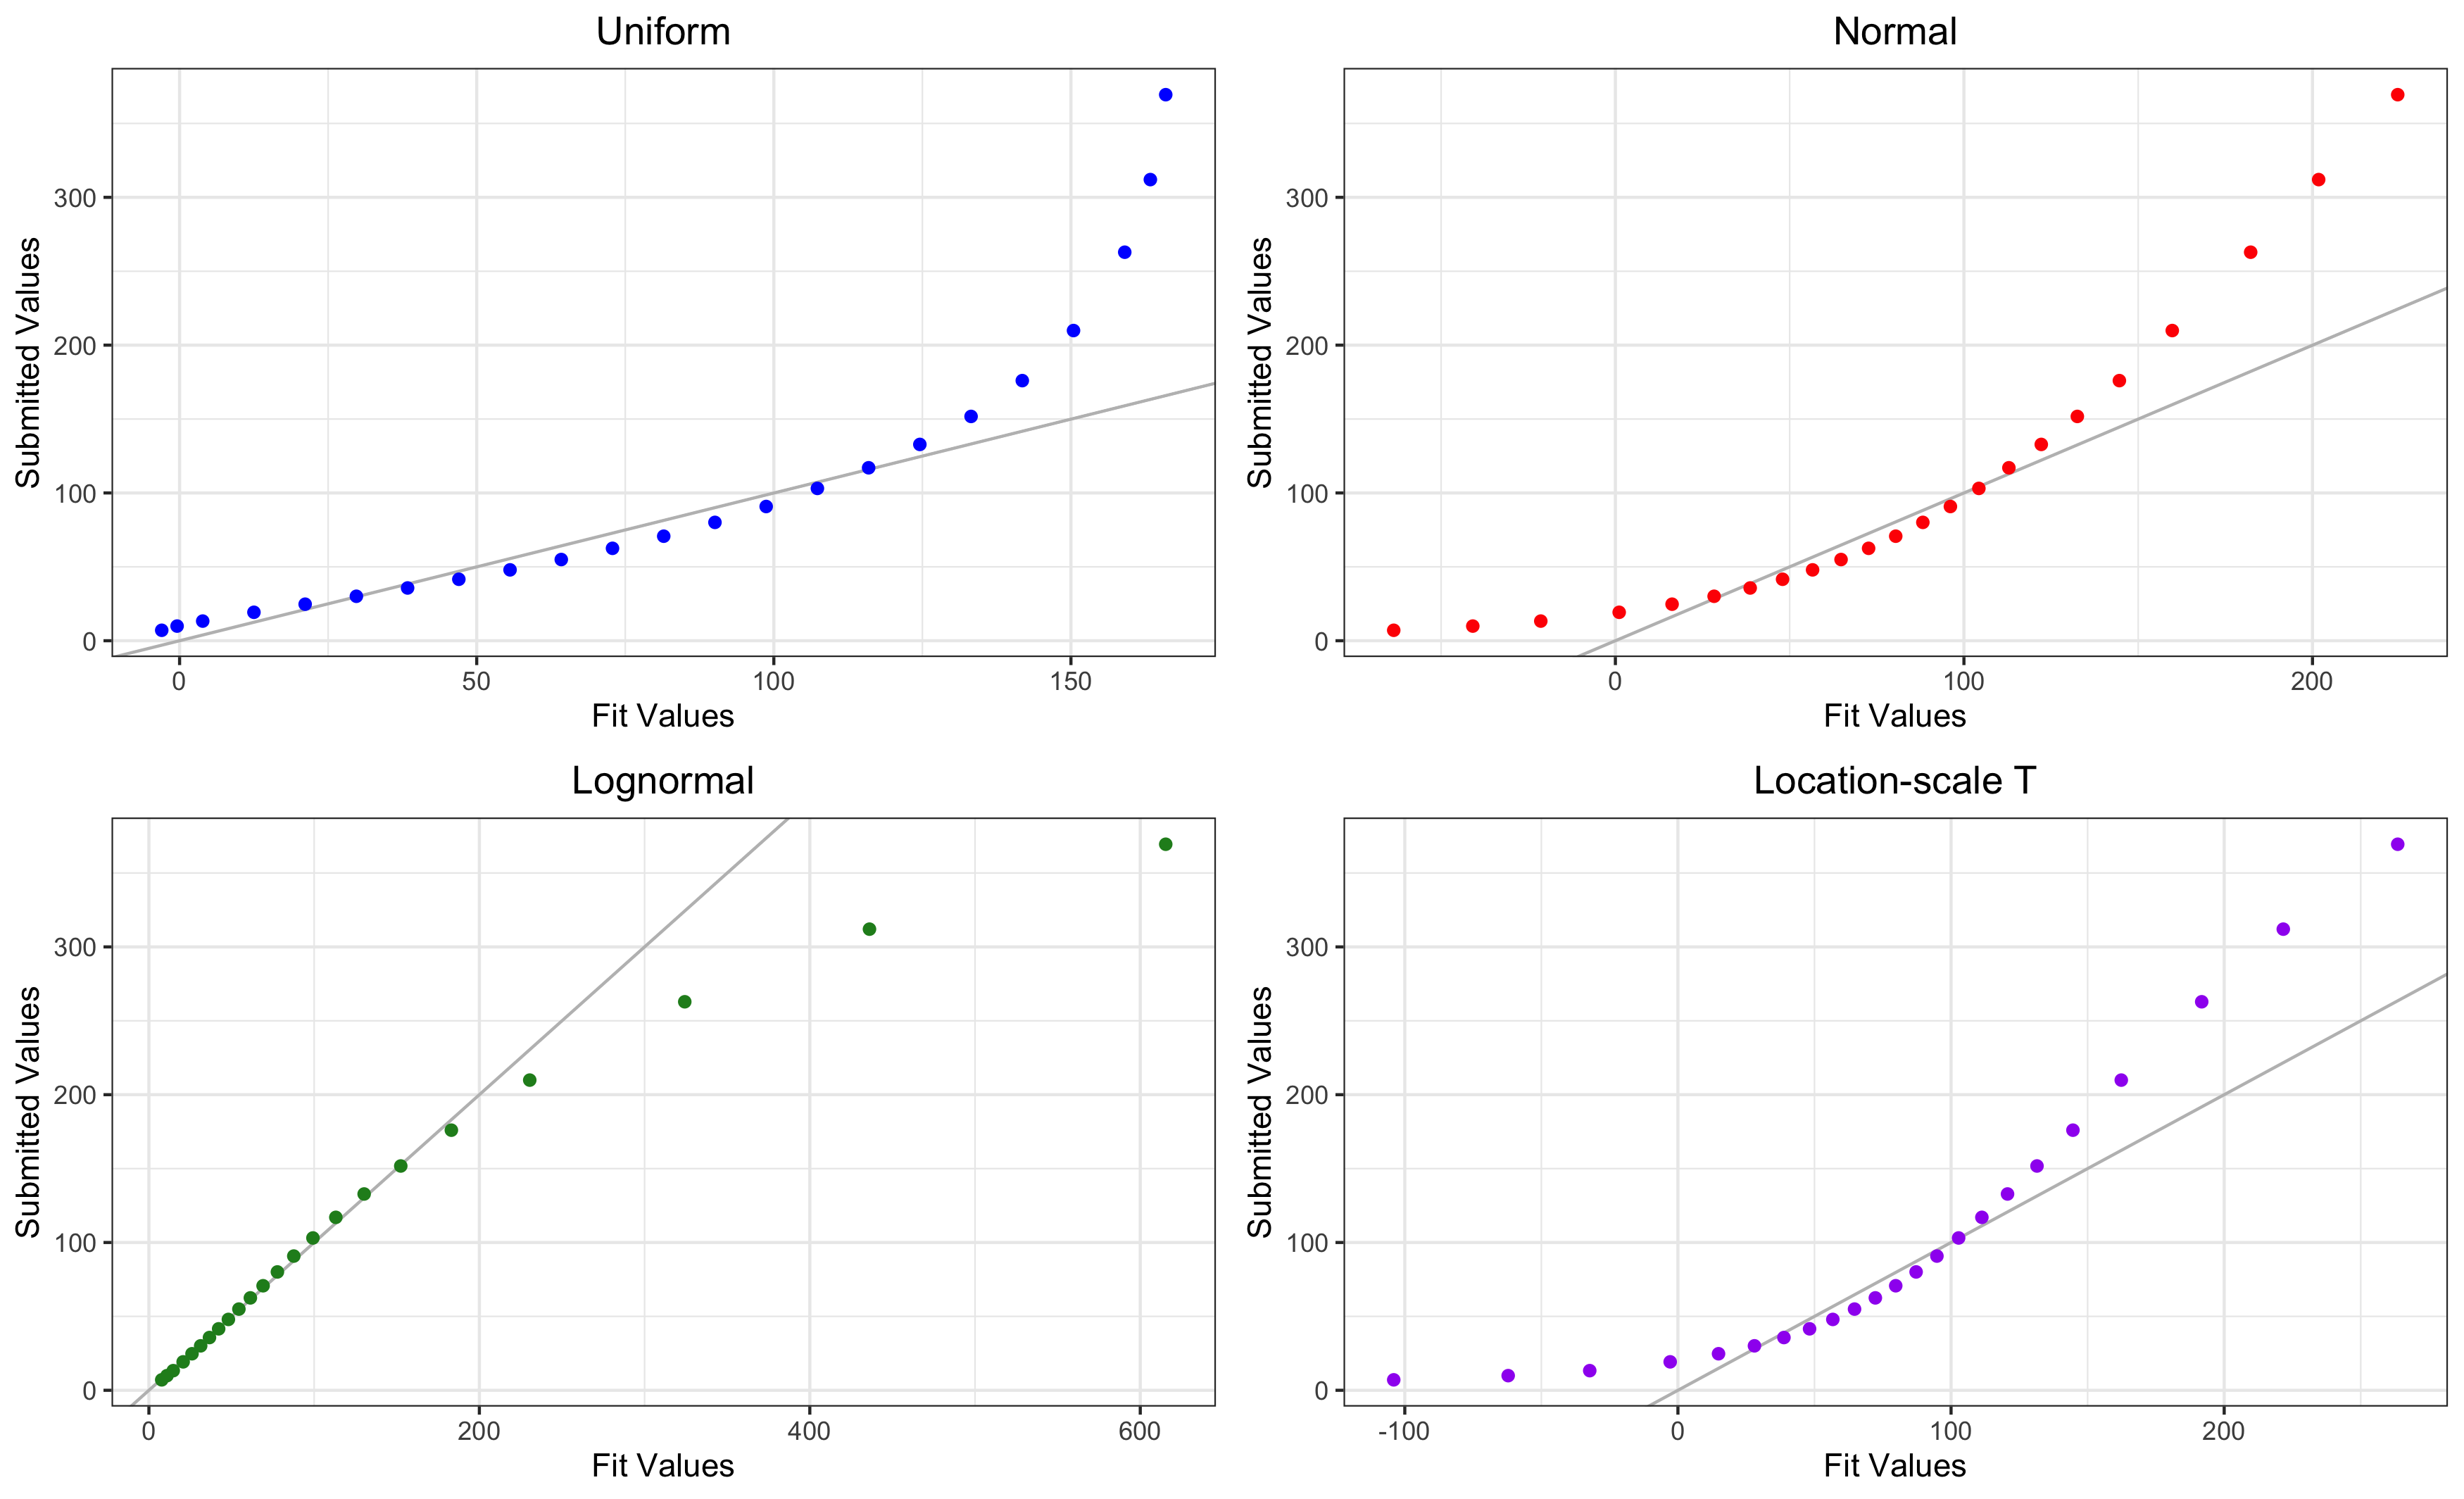
\includegraphics[scale=.15]{Images/qq_gleam_110121_1wkincdeath_st16.png}}
\begin{center}
\begin{minipage}{10cm}
\captionsetup{font=scriptsize}
\caption[QQ plot for quantile fit]{This figure shows qq plots for a set of
submitted quantiles against the quantiles the continuous distribution to which
it was fit. 
The name of this forecast given by the team who submitted it is Gleam COVID-19.
This forecast was submitted to the C0VID-19 Forecast Hub on November 1, 2021
and is forecasting deaths one in the next week in a certain US state due to the
virus.
In no case here was the MSE below the cutoff value of the 
corresponding distribution.}
\label{fig:qqfits}
\end{minipage}
\end{center}
\end{figure}

\begin{figure}[htbp]
\centerline{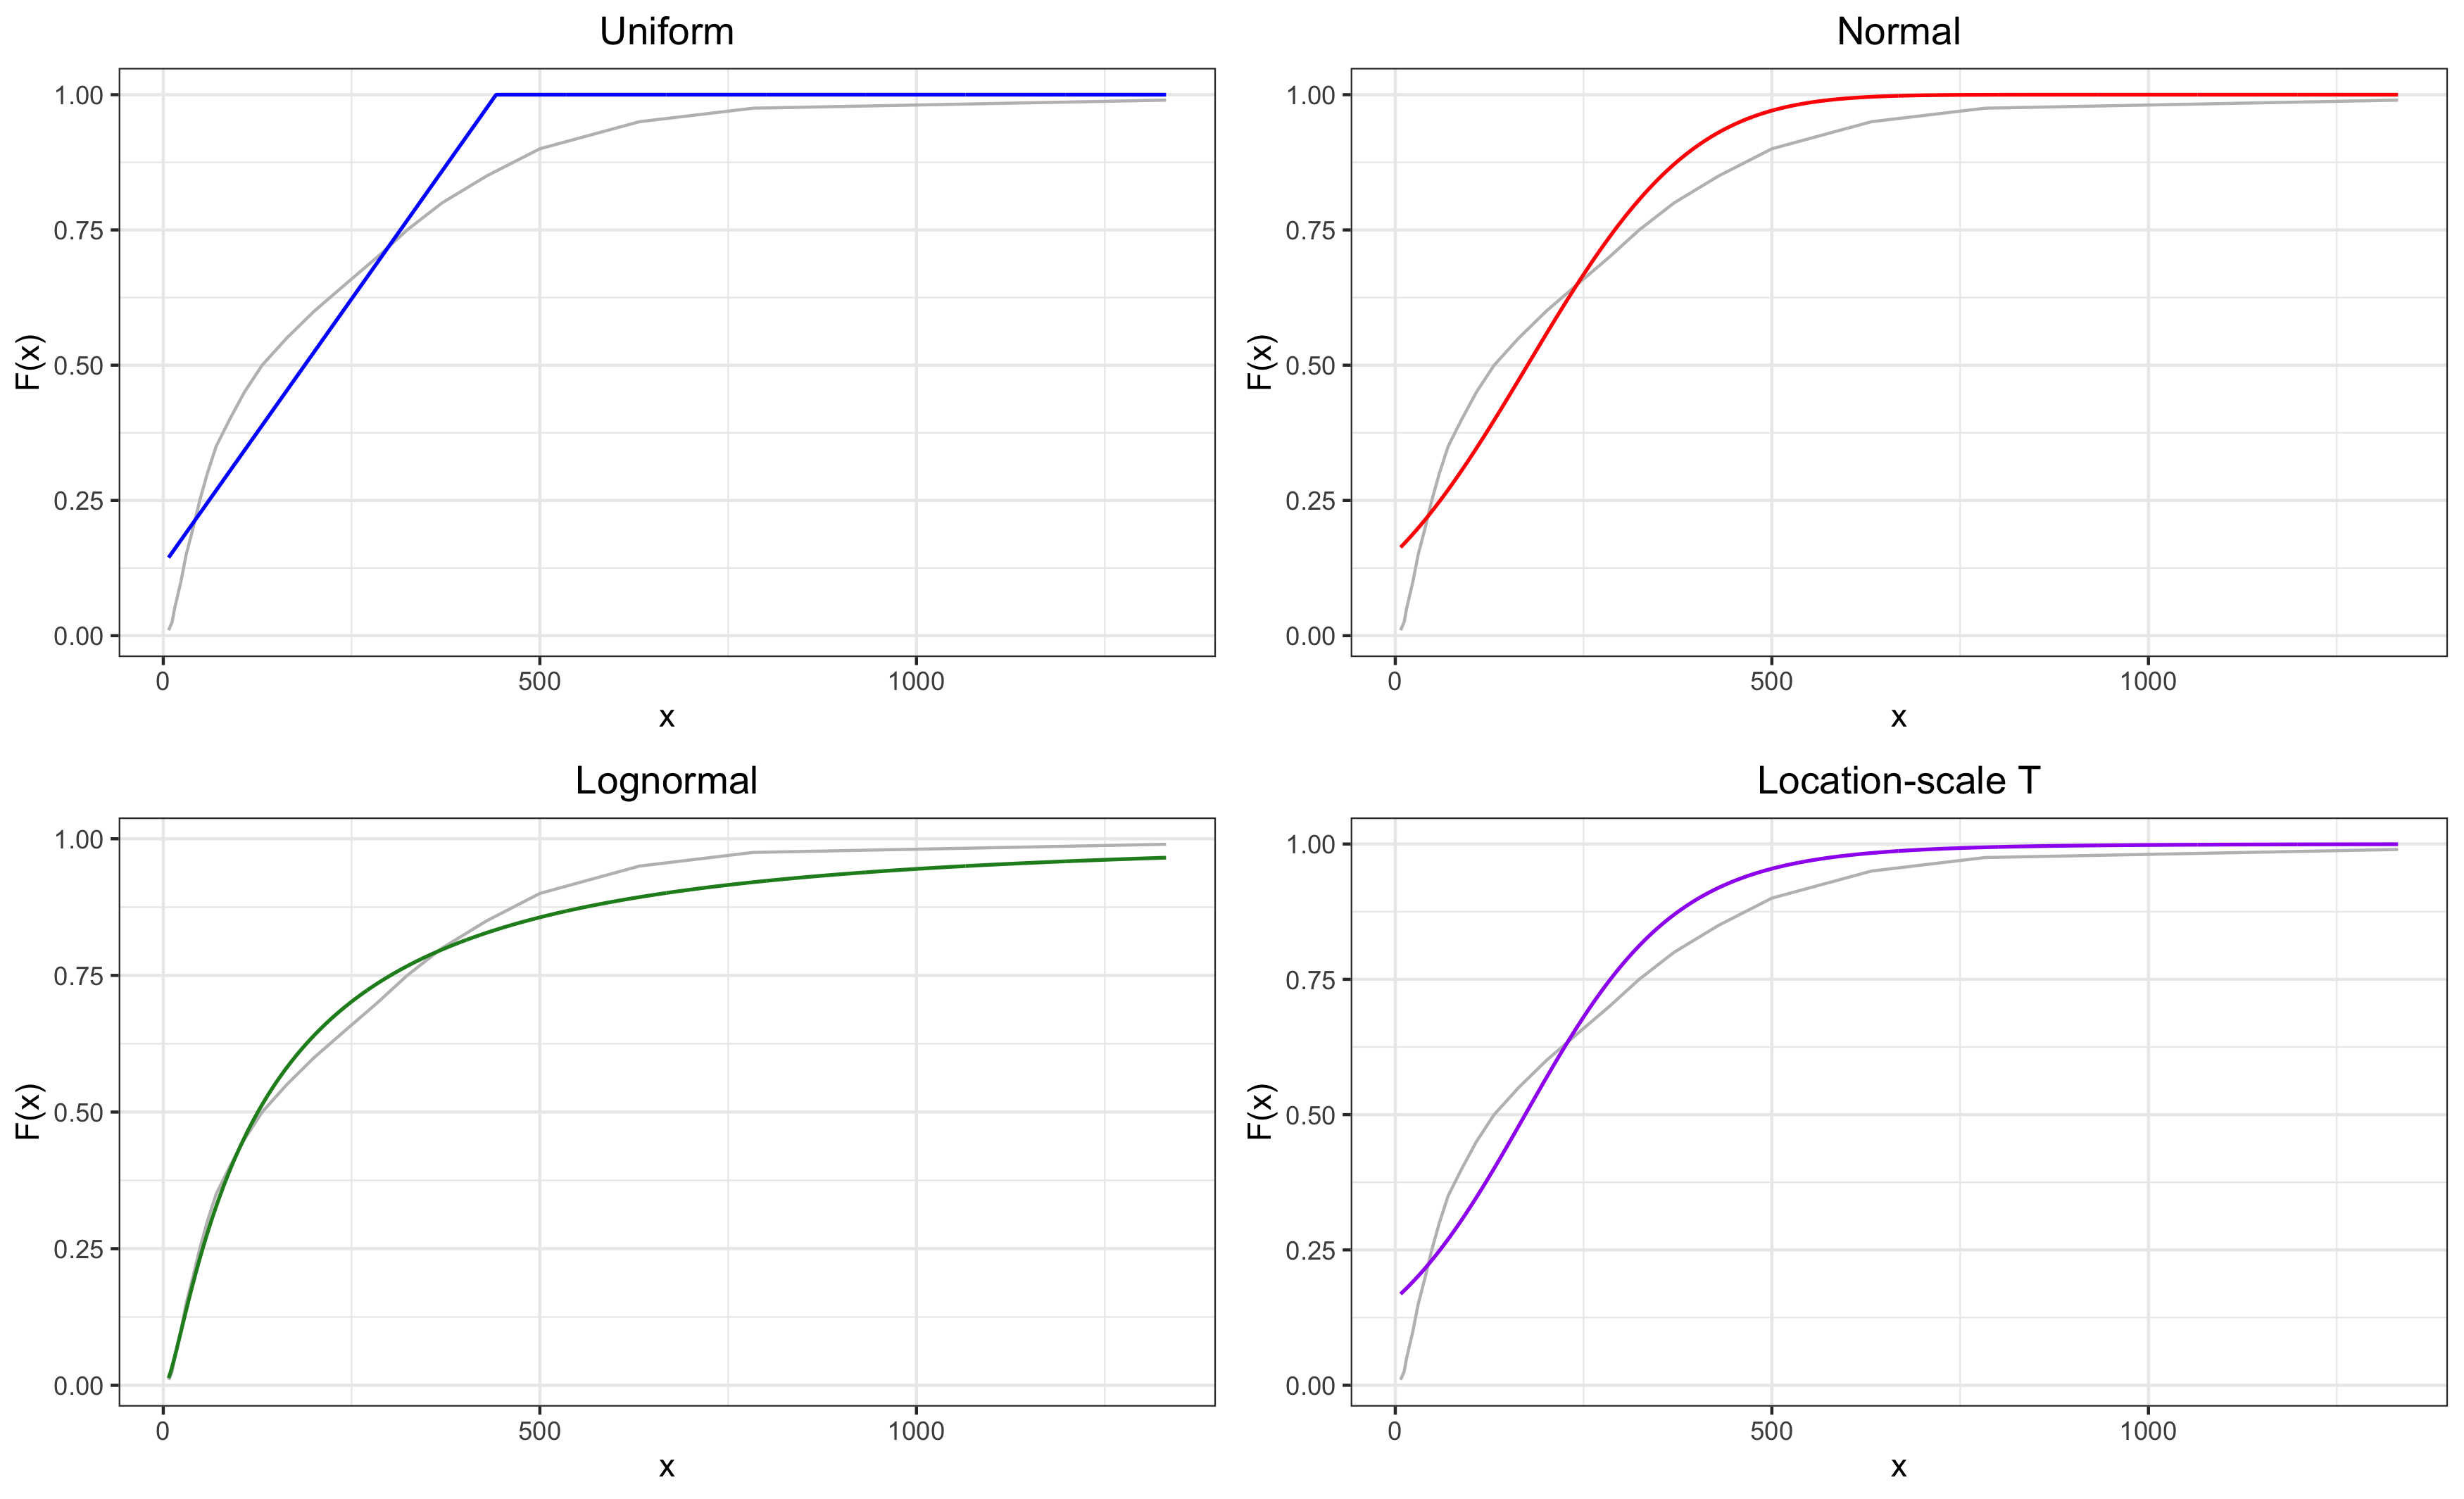
\includegraphics[scale=.15]{Images/cdf_gleam_110121_1wkincdeath_st16.png}}
% i=11,j=12,k=5
\begin{center}
\begin{minipage}{10cm}
\captionsetup{font=scriptsize}
\caption[CDF plot for quantile fit]{This figure shows the CDF plots for 
distributions fit to a set of quantiles. The grey line is a line of connected 
dots from the submitted quantiles and values and is the same in all four plots.
This is the same set of forecasts as is \ref{fig:qqfits}.
In no case here was the MSE below the cutoff value of the 
corresponding distribution.}
\label{fig:cdffits}
\end{minipage}
\end{center}
\end{figure}



The results from these two studies suggest that in some cases, forecasters
are using methods which produce may produce one component mixture distribution
forecasts. Many
likely are not. To expand upon these studies, one could attempt to fit the 
bin forecasts or the quantile forecasts to mixture 
distributions with multiple components. Forecasts that are very close to 
a mixture distribution may suggest that the forecasters already have models that
make transition to a mixture distribution forecast format easy or
straightforward.

















\chapter{Discussion}

In this paper we have reviewed four representation types commonly used in
probabilistic 
forecasting including proper scoring, data storage, and ensemble model 
construction for each type. We presented the mixture distribution
representation and we argue that its use in collaborative probabilistic 
forecasting is preferable to the other representations.
In terms of model flexibility, storage, and 
ensemble building it is
comparable to discretized bins and quantile forecasts but also provides a 
forecast with a infinite nominal resolution. Based on a retrospective analysis,
we argue that among the teams participating in the CDC flu
competition and the COVID-19 Forecast Hub, there are already some which produce
forecasts already resembling single component mixture distributions making the 
transition from past and current formats to a mixture distribution format 
straightforward.
We thus advocate for the use of mixture distributions in
future forecasting projects like those done in the CDC flu competition or in the
COVID-19 Forecast Hub.

For a number of reasons, the adoption of mixture distributions as the
submission format may be avoided. A collaborative forecast center, along with 
forecasters, using a 
different representation may simply not want to break from tradition. The 
implementation of new scoring and ensemble construction methods may be a 
barrier. Development of tools beyond what was used in Section 
\ref{section:tools} would assist in making a transition to using mixture 
distributions more straightforward.
One aspect of ensemble construction which received little attention in 
this paper is the selection of weights for components of an ensemble where each
of the components is mixture distribution. Computing requirements could become a
concern in such a problem and further research on this may provide
ideas of best methods for weight selection.

Another area of recommended research is the use of joint mixture distributions 
for 
forecasting. We have only considered here probabilistic forecasting of one 
event at a time. Number of new infections in one week at one specific location
for example. This forecast is presented as a marginal distribution for that 
specific target, time, and location. A joint distribution for forecasting 
multiple targets, times or locations may sometime be desirable and may require
further consideration on how joint mixture distributions could be used as a 
format in collaboration.






















% \include{Body/ch1/ch1_main}
% \include{Body/ch2/ch2_main}
% \include{Body/ch3/ch3_main}
% \include{Body/ch4/ch4_main}
% \include{Body/ch5/ch5_main}
%\include{Body/ch6/ch6_future_and_conclusions}


%\bibliographystyle{acm} % use for numbered citations along with options given in preamble. Look at the main thesis.tex file


% \bibliographystyle{apa}
% \bibliography{master_bib}

% \section{Bibliography}
% \bibliographystyle{apa}
% % \vspace{-20pt}
% \begingroup
%     \setlength{\bibsep}{13.2pt}
%     \linespread{1}\selectfont
%     \bibliography{master_bib}
% \endgroup
% \clearpage
% \pagebreak

%%%%%% bibliographies

\clearpage
\nocite{*}
\unappendixtitle
\newpage
\phantomsection
\addcontentsline{toc}{chapter}{BIBLIOGRAPHY}
\section*{BIBLIOGRAPHY}
\bibliographystyle{apa}
\vspace{-20pt}
\begingroup
   \setlength{\bibsep}{14.5pt}
   \linespread{1}\selectfont
\bibliography{master_bib}
\endgroup

\appendix

\specialchapt{APPENDIX}
\label{section:append}


The following is the code to make the \texttt{MakeDist()} function introduced 
in \ref{section:tools}.
\begin{Schunk}
\begin{Sinput}
> MakeDist <- function(distsdf){
+   
+   distdf <- distsdf[distsdf[,1] != 'Lst',]
+   tdist <- distsdf[distsdf[,1] == 'Lst',]
+   
+   fun_dist <- 
+     apply(distdf, FUN=function(x) {
+       paste('distr::',x[1], '(', 
+             ifelse(!is.na(x[2]) & (!is.na(x[3]) | !is.na(x[4])),
+                    paste(x[2],',',sep=''),
+                    ifelse(!is.na(x[2]) & is.na(x[3]) & is.na(x[4]),
+                           x[2], '')), 
+             ifelse(!is.na(x[3]) & !is.na(x[4]),
+                    paste(x[3],',',sep=''),
+                    ifelse(!is.na(x[3]) & is.na(x[4]), x[3],'')), 
+             ifelse(!is.na(x[4]),x[4],''), ')',sep='')
+     }, MARGIN = 1
+     )
+   
+   fun_tdist <- apply(tdist, FUN=function(x) {
+     paste0('distr::Td(',x[4],')*',x[3], '+', x[2])
+   }, MARGIN = 1
+   )
+   
+   dist_args <- paste(fun_dist, collapse=',',sep='')
+   tdist_args <- paste0(fun_tdist,collapse=',')
+   args <- ifelse(tdist_args!='',paste(dist_args,tdist_args,sep=','),dist_args)
+   
+   weights <- c(distdf[,5],tdist[,5])
+   mixString <- paste('distr::UnivarMixingDistribution(',
+                      args,',mixCoeff=weights)',sep='')
+   mixDist <- eval(parse(text=mixString))
+   
+   return(mixDist)
+ }
\end{Sinput}
\end{Schunk}


The following is the code used to make the function \texttt{CRPS()} used in
section \ref{section:tools}.
\begin{Schunk}
\begin{Sinput}
> crps_integrand <- function(x,dist,y) {(dist(x) - as.numeric(y <= x))^2}
> CRPS <- function(y,dist) {
+   int <- integrate(crps_integrand,-Inf,Inf,y,dist=dist)
+   return(int$value)
+ }
\end{Sinput}
\end{Schunk}





% Renders the citations but does not show the bibliography at the end of the thesis
%\newsavebox\mytempbib
%\savebox\mytempbib{\parbox{\textwidth}{\bibliography{master_bib}}}

\clearpage
\pagebreak

%% Only within chapter appendix is allowed for Journal style writing
%% Appendix1 file from standard thesis template

\appendixtitle 
\appendix


%% Use the following two lines for single appendix
%\unappendixtitle
%\singleappendixtitle

% Please note the appendix can be removed if the thesis does not require an overall appendix

\chapter{ADDITIONAL MATERIAL} 
This is now the same as any other chapter except that
all sectioning levels below the chapter level must begin
with the *-form of a sectioning command.

\section*{More stuff}

Supplemental material.

 % Instruction for single appendix look below
%% An example second appendix from the example thesis thesis.tex.
\chapter{STATISTICAL RESULTS}

This is now the same as any other chapter except that
all sectioning levels below the chapter level must begin
with the *-form of a sectioning command.

\section*{Supplemental Statistics}

More stuff.

\end{document}

% use \isucaption{} for all captions of figures and tables, where the captions are not too long.

% Use \isucaption[]{} with the square brackets for short caption of figure or table that goes into the list of tables and list of figures, and the curly brackets can have long captions which go with the figure/ table.

% IMPORTANT NOTES
% TABLE OF CONTENTS :
% TOPIC 1:  If you need a page break follow the steps below
% step1
% check before which chapter in the table of contents you want a page break
% step 2
% go the folder "body". There open the chapter tex file that you noted needed page break in the table of contents..
% step 3
% insert  \addtocontents{toc}{\protect\newpage} before the first line i.e. before the line \chapter{RESULTS}.

%%%%%%%%%%%%%%
% use \isucaption{} for all captions of figures and tables, where the captions are not too long.

% Use \isucaption[]{} with the square brackets for short caption of figure or table that goes into the list of tables and list of figures, and the curly brackets can have long captions which go with the figure/ table.

%%%%%% Using sub figures 
% %%% In preamble include : \usepackage{subfig}
% \begin{figure}[htbp]
% 	\centering
% 	\subfloat[first caption.\label{fig:2a}]{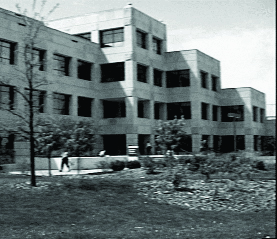
\includegraphics[width=0.2\textwidth]{Images/dc5.jpg}}\hfill
%     \subfloat[second caption.\label{fig:2b}] {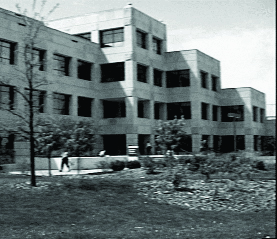
\includegraphics[width=0.2\textwidth]{Images/dc5.jpg}}\hfill
% 	\isucaption{Sub-figure test}
% 	\label{fig:subfigure-test}
% \end{figure}

% Subfloat reference: Fig \ref{fig:2a}

% Figure reference: Fig \ref{fig:subfigure-test}
